% !TeX program = xelatex
% !TeX encoding = UTF-8
% 中文写作稿；底稿：paper-v2-bak.tex（与创建时 paper-v2 copy.tex 相同）。
% 保留原稿公式、引用键和实验图资源；图内已有英文标注暂沿用。
% 编译：latexmk -xelatex -interaction=nonstopmode paper-zh.tex
%%
%% 中文写作稿（沿用 ACM 双栏布局）
%%
\documentclass[sigconf,balance=false]{acmart}
\usepackage[UTF8,scheme=plain,fontset=fandol]{ctex}
\usepackage{etoolbox}
% 仅本中文稿使用中文名称；保留 acmart 的计数器及原排版结构。
\AtBeginDocument{%
  \renewcommand{\abstractname}{摘要}%
  \renewcommand{\refname}{参考文献}%
  \renewcommand{\proofname}{证明}%
  \patchcmd{\theorem}{Theorem}{定理}{}{}%
  \patchcmd{\lemma}{Lemma}{引理}{}{}%
  \patchcmd{\definition}{Definition}{定义}{}{}%
}

\AtBeginDocument{%
  \providecommand\BibTeX{{Bib\TeX}}}

\setcopyright{none}
\settopmatter{printacmref=false}
\acmYear{2026}
\acmConference[Anonymous Submission]{Anonymous Submission}{2026}{Venue withheld for review}
\acmBooktitle{Anonymous Submission}
\acmDOI{}
\acmISBN{}

\usepackage{hyperref}
\usepackage{url}
\usepackage{booktabs}
\usepackage{amsfonts}
\usepackage{amsmath}
\usepackage{bm}
\usepackage{algorithm}
\usepackage{algpseudocode}
\floatname{algorithm}{算法}
\algrenewcommand\algorithmicrequire{输入：}
\algrenewcommand\algorithmicensure{输出：}
\algrenewcommand\algorithmicreturn{返回}
\algrenewcommand\algorithmicif{若}
\algrenewcommand\algorithmicthen{则}
\algrenewcommand\algorithmicelse{否则}
\algrenewcommand\algorithmicfor{对于}
\algrenewcommand\algorithmicdo{执行}
\algrenewcommand\algorithmicwhile{当}
\algrenewcommand\algorithmicend{结束}
\usepackage{graphicx}
\usepackage{enumitem}
\usepackage{placeins}
\usepackage{balance}
\usepackage{microtype}
\usepackage{xcolor}
\usepackage{tikz}
\usetikzlibrary{arrows.meta,backgrounds,calc,fit,positioning}

\definecolor{cimTeal}{HTML}{1F6F78}
\definecolor{cimGold}{HTML}{C28B2C}
\definecolor{cimRed}{HTML}{A95050}
\definecolor{cimBlue}{HTML}{496F9B}
\definecolor{cimGray}{HTML}{667078}
\definecolor{cimLight}{HTML}{F3F5F5}
\tikzset{
  cimnode/.style={circle,draw=cimGray,fill=white,minimum size=5.8mm,
                  inner sep=0pt,font=\scriptsize},
  cimseed/.style={cimnode,draw=cimBlue,very thick,fill=cimBlue!10},
  cimadopt/.style={cimnode,draw=cimTeal,very thick,fill=cimTeal!13},
  cimdrop/.style={cimnode,draw=cimRed,very thick,fill=cimRed!10},
  cimset/.style={rounded corners=2pt,draw=cimGray,fill=cimLight,
                 inner xsep=5pt,inner ysep=4pt,font=\scriptsize},
  cimarrow/.style={-{Latex[length=2mm]},semithick,cimGray},
  cimlabel/.style={font=\scriptsize,align=center}
}

\newcommand{\CIMRIS}{\textsc{CIM-RIS}}
\newcommand{\E}{\mathbb{E}}
\newcommand{\I}{\mathbb{I}}

\begin{document}

\title{不可复制扩散下的优惠券影响力最大化}

\author{匿名作者}

\renewcommand{\shortauthors}{匿名作者}

\begin{abstract}
经典影响力最大化假设信息可以复制，并从一个已激活用户分支传播给多个邻居。
数字优惠券则作为不可复制的对象流转：接收者可以核销、丢弃，或将其转发给一个邻居，且只有核销才产生采纳用户。
本文将这一场景形式化为优惠券影响力最大化（Coupon Influence Maximization，CIM）问题，即分配有限数量、独立扩散的优惠券，以最大化不同核销用户数的期望。
我们证明 CIM 是 NP-hard 的，并证明采纳规模在整数优惠券分配上具有单调性和边际收益递减性质。
因此，精确贪心算法可获得 $(1-1/e)$ 近似比，但其边际收益计算代价较高。
为此，我们提出保留优惠券身份的 $k$ 联合反向可达样本，将根节点采纳与反向可达性分离，并利用覆盖事件构造采纳规模和边际收益的无偏估计量。
在此基础上，\CIMRIS{} 以高概率返回 $(1-1/e-\epsilon)$ 近似分配；当预算、精度和采纳规模下界固定时，其期望运行时间关于图规模近线性。
在五个存档网络图实例上进行的实验评估了该方法的解质量与实际可扩展性。
在具有高精度蒙特卡洛贪心参考结果的两个图、三种场景中，观察到的差距为 $0.3$--$11.1\%$；在 Netscience 上为 $1.1$--$4.4\%$。
\CIMRIS{} 在全部 72 个图--场景--预算配置中均优于度数和 PageRank 基线；在计入根生成的补充测量中，$k=10$ 时条件根采样在 Netscience 和 EmailEnron 上分别带来约 $1.20\times$ 和 $1.37\times$ 的方差--时间效率提升。
完整 Douban 的补充独立评估中，\CIMRIS{} 在六个预算中的五个略低于随机投放，表明固定经验采样预算下的解质量优势具有条件性。
\end{abstract}

\begin{CCSXML}
<ccs2012>
 <concept>
  <concept_id>10002951.10002952.10002953.10010820</concept_id>
  <concept_desc>Information systems~Social networks</concept_desc>
  <concept_significance>500</concept_significance>
 </concept>
 <concept>
  <concept_id>10003752.10003809.10010170.10010171</concept_id>
  <concept_desc>Theory of computation~Approximation algorithms analysis</concept_desc>
  <concept_significance>300</concept_significance>
 </concept>
</ccs2012>
\end{CCSXML}

\ccsdesc[500]{Information systems~Social networks}
\ccsdesc[300]{Theory of computation~Approximation algorithms analysis}

\keywords{影响力最大化，优惠券扩散，随机游走，反向影响力采样，次模优化}

\maketitle

\hypersetup{
  pdftitle={不可复制扩散下的优惠券影响力最大化},
  pdfauthor={匿名作者},
  pdfkeywords={影响力最大化，优惠券扩散，随机游走，反向影响力采样，次模优化}
}

%% ============================================================
%% 1. INTRODUCTION
%% ============================================================
\section{引言}
\label{sec:intro}

口碑传播和病毒式营销是在线社交网络中促进用户采纳产品的重要策略。
影响力最大化（Influence Maximization，IM）研究如何选择有限数量的种子用户，使其扩散过程激活尽可能多的用户~\cite{kempe2003maximizing}。
过去二十余年中，独立级联（Independent Cascade，IC）和线性阈值（Linear Threshold，LT）模型下的 IM 得到了广泛研究；在这些模型中，已激活用户可以影响多个邻居，从而形成分支级联~\cite{domingos2001mining,borgs2014maximizing,tang2015influence}。
然而，许多促销对象不可复制，无法用这种广播假设描述。
例如，一张数字优惠券可以被核销、丢弃或转发给一位好友，却不能同时复制给多个邻居。
因此，它的扩散轨迹类似于随机游走路径，而非级联。

考虑一家企业通过社交网络发放 $k$ 张数字优惠券。
用户收到优惠券后，可以核销、丢弃，或将其转发给一个出邻居。
核销和丢弃均终止该券的扩散；转发则将同一张券交给下一位用户，不会产生副本。
只有核销至少一张券的用户才被计为采纳用户；仅转发优惠券的用户不贡献目标收益。
不同优惠券独立扩散，同一用户可能核销多张券，但只被计数一次。
企业也可以向同一初始用户分配多张券，因为从该用户出发的独立优惠券可能沿不同路径传播。

上述机制产生了有别于经典 IM 的种子分配问题。
将多张券投给单券表现较好的种子，可能使传播轨迹在同一批采纳用户处重叠；选择较差的种子，则可能导致大量优惠券被丢弃。
据此，我们定义\emph{优惠券影响力最大化}（CIM）：给定 $k$ 张券的预算，将其分配给种子用户，使不同核销用户数的期望最大。
我们还将优惠券使用率，即已发放优惠券中最终被核销的比例的期望，作为补充性的活动指标。

本文形式化描述优惠券扩散过程，并研究 CIM 的计算性质与结构性质。
我们证明 CIM 是 NP-hard 的，并证明其采纳规模目标在优惠券分配上具有边际收益递减性质。
这一性质支持贪心分配策略，但在大规模网络上，通过前向蒙特卡洛模拟直接计算边际收益的代价过高。
受反向影响力采样（Reverse Influence Sampling，RIS）启发，我们构造优惠券感知的反向可达（Reverse Reachable，RR）样本，将边际收益估计转化为覆盖计算。
由此得到的 \CIMRIS{} 算法以高概率实现 $(1-1/e-\epsilon)$ 近似比。

CIM 与经典 IM 在模型和算法两个层面均存在差异。
在 IC 和 LT 中，激活与传播相互耦合：已激活用户可以继续向多个邻居传播级联。
在 CIM 中，传播沿单一路径进行，中间转发者仍不是采纳用户。
在算法层面，本文的联合 RR 构造保留每张券的独立实现及其索引，以避免不同券之间的错误匹配。
经典广播模型的 RR 生成过程不能原样用于该传播机制，但在建立正确的优惠券覆盖估计器后，仍可利用通用次模优化方法。

本文的贡献主要包括三个方面。
第一，提出优惠券影响力模型并形式化定义 CIM，刻画不可复制的单路径扩散、优惠券之间的独立性以及采纳用户重叠。
第二，证明 CIM 的 NP-hard 性，并建立采纳规模在整数分配上的边际收益递减性质，从而在边际收益可精确计算时支持 $(1-1/e)$ 贪心近似。
第三，提出优惠券感知的 RR 采样和可扩展的 \CIMRIS{} 算法，通过估计边际收益，以高概率保持 $(1-1/e-\epsilon)$ 近似保证。
在五个存档网络图实例上，我们评估了解质量、可扩展性、采样预算敏感性、容量约束下的分配，以及条件根采样带来的方差降低。
具体而言，\CIMRIS{} 的解质量与蒙特卡洛贪心具有可比性，持续优于仅依赖拓扑的种子排序；在采用固定经验采样预算时，它在含 154,907 个节点的 Douban 实例上选择 200 个种子耗时 31.2 秒。
该预算下的独立大图质量评估未显示其对所有已测基线的优势；经验采样预算也不构成理论近似保证的单次运行证书。

%% ============================================================
%% 2. RELATED WORK
%% ============================================================
\section{相关工作}
\label{sec:related}

\textbf{影响力最大化。}
早期研究将病毒式营销建模为社交网络上的优化问题~\cite{domingos2001mining,richardson2002mining}。
Kempe 等~\cite{kempe2003maximizing} 在 IC 和 LT 模型下形式化定义 IM，证明其 NP-hard 性，并利用单调性和次模性得到 $(1-1/e)$ 贪心近似。
后续工作通过惰性贪心及针对具体模型的优化加速边际收益计算~\cite{leskovec2007celf,goyal2011celf,chen2009efficient}。
通用随机贪心还可通过抽取候选元素减少单调次模最大化的目标函数调用次数~\cite{mirzasoleiman2015lazier}。
这些优化框架可用于本文的目标；需要另外解决的是单次目标或边际收益评估的成本。
这些模型描述的是可复制的影响力：已激活节点能够尝试激活多个邻居。
CIM 分配的则是不可复制的优惠券，每张券仅沿一条路径转发，并且只有用户核销时才产生采纳。

\textbf{反向影响力采样。}
Borgs 等~\cite{borgs2014maximizing} 提出 RR 集方法，将影响力估计转化为随机集合覆盖。
TIM/TIM+~\cite{tang2014influence}、IMM~\cite{tang2015influence}、Stop-and-Stare~\cite{nguyen2016stop,huang2017revisiting} 和 OPIM-C~\cite{tang2018online} 逐步提升了这一框架的理论效率与实际效率。
其基本覆盖事件是种子集与一次广播实现所生成的 RR 集相交。
本文的反向构造有两点不同：根节点采纳被单独建模为门控事件；每个样本包含分别对应各张券的独立 RR 分量。
在本文的联合样本中，覆盖判定必须保持券索引的一致性；该要求不排除采用其他正确的估计器或优化框架。

\textbf{优惠券与激励分配。}
Yang 等~\cite{yang2016continuous} 研究通过连续折扣控制用户成为种子的概率，以在预算内最大化期望影响力。
该问题通常也缩写为 CIM；本文的 CIM 特指 Coupon Influence Maximization，其决策变量是不可复制优惠券的整数投放数量，而非折扣水平。
Tang~\cite{tang2018coupon} 研究离散券面额分配，以近似次模效用描述后续级联，并考虑 matroid 和预算约束；同一用户收到多张券时，其采纳概率由最高面额决定。
Chang 等~\cite{chang2019socialcoupon} 在带推荐配额的 IC 扩展中联合选择种子和内部节点的优惠券资源，以期望激活收益与种子及优惠券成本之比为目标。
该比值不同于本文定义的优惠券使用率 $\eta=\rho/k$。
这些研究说明，优惠券分配并非新的应用主题；本文研究的是单券转交、核销即终止及独立多券终点去重的具体传播机制。
在本文模型中，转发本身不产生采纳收益，同一用户接收不同券时分别作出独立决策。
因此，已有研究的传播和收益计算不能不经转换直接替代本文的估计过程；通用次模优化工具则仍然适用。

\textbf{扩散模型变体。}
已有研究还考察了竞争扩散、虚假信息控制、位置约束、自适应种子选择和多轮活动下的 IM~\cite{budak2011limiting,li2014efficient,lu2015competition,seeman2013adaptive,sun2018multi}。
Liao 等~\cite{liao2023popularity} 则以优惠券发放为动机，在多轮活动中分配促销种子，以提高产品的流行度比率。
不过，其 PA-IC 模型仍通过 IC 级联传播可复制的促销信息，并未将每张优惠券建模为被转发和消耗的单一对象。
随机游走为图上的单路径移动提供了经典基础~\cite{lovasz1993random}，但标准随机游走目标未同时刻画终止性采纳、不可复制性以及独立发放优惠券之间的采纳重叠。
CIM 将这些特征纳入统一优化模型，并为其构造优惠券感知的反向采样器。

%% ============================================================
%% 3. MODEL AND PROBLEM DEFINITION
%% ============================================================
\section{模型与问题定义}
\label{sec:model}

本节介绍优惠券影响力模型，将不可复制优惠券与社交网络中的单路径、类随机游走传播相结合。
随后定义优惠券影响力最大化（CIM）问题：向初始接收者分配 $k$ 张券，以最大化不同采纳用户数的期望。

\subsection{优惠券影响力模型}

经典 IM 通常在独立级联（IC）和线性阈值（LT）模型下研究~\cite{kempe2003maximizing}。
在时间步 $0$，所有种子节点被激活，其余节点未激活；节点一旦激活便保持激活状态。
在 IC 中，于时间步 $i$ 激活的节点在 $i+1$ 时有一次机会，按照连接边上的传播概率独立尝试激活每个尚未激活的出邻居。
在 LT 中，每个节点独立从 $[0,1]$ 选择阈值，当已激活入邻居的权重总和达到该阈值时被激活。
当不再有节点可被激活时，传播终止。
可扩展 IM 算法通常采用反向影响力采样（RIS）求解这一问题~\cite{borgs2014maximizing,tang2015influence}。
生成一个随机反向可达（RR）集时，先从 $V$ 中均匀采样根节点，再反向追踪随机扩散实现中所有能够激活该根的节点。
任意种子集 $S$ 的期望影响力等于 $n\Pr[S\cap R\neq\emptyset]$，因此 IM 可转化为采样 RR 集上的最大覆盖问题。
给定 $\theta$ 个独立 RR 集，$S$ 覆盖的比例既是其归一化影响力的极大似然估计，也是无偏估计。
所需 $\theta$ 通常结合最优影响力下界的估计与集中不等式自适应确定，然后通过贪心算法选择边际 RR 覆盖最大的 $k$ 个节点。
CIM 沿用这一总体优化思路，但单路径、不可复制的扩散语义要求不同的 RR 集生成过程及覆盖问题。

将社交网络建模为有向图 $G=(V,E)$，其中 $V$ 为 $n=|V|$ 个用户组成的集合，$E$ 为 $m=|E|$ 条有向转发关系组成的集合。
记 $V_s\subseteq V$ 为可选种子用户集合；所有用户均可作为种子时，令 $V_s=V$。
每个 $v\in V_s$ 具有投放容量 $c_v\in\{1,\ldots,k\}$。
$c_v=1$ 要求种子互不相同，$c_v=k$ 则允许将全部优惠券投给同一用户。
假设 $\sum_{v\in V_s}c_v\geq k$。
每个节点 $u\in V$ 具有采纳概率 $p_u^a$、丢弃概率 $p_u^d$ 和转发概率 $p_u^t$，满足 $p_u^a+p_u^d+p_u^t=1$。
本文中“采纳”具体指核销优惠券，采纳用户即核销用户。
对每条边 $(u,v)\in E$，$p(u,v)$ 表示 $u$ 将优惠券转发给 $v$ 的无条件概率，因此 $\sum_{v:(u,v)\in E}p(u,v)=p_u^t$。
没有出邻居的节点须满足 $p_u^t=0$。

考虑一张投放于 $s\in V_s$ 的优惠券。
在时间步 $0$，节点 $s$ 持有该券。
若节点 $u$ 在时间步 $\tau$ 持有该券，则以概率 $p_u^a$ 核销并成为采纳用户，或以概率 $p_u^d$ 丢弃；这两种行为均终止该券的扩散。
否则，$u$ 以概率 $p(u,v)$ 将券转发给出邻居 $v$，由 $v$ 在时间步 $\tau+1$ 持有。
因此，一张券产生一条转发路径，而非分支级联。

在这一过程中，传播与采纳相互分离。
转发者可以帮助优惠券抵达后续采纳用户，但自身并不因此成为采纳用户；用户只有核销优惠券才贡献目标收益。
经典 IC 和 LT 扩散中没有这一分离，因为已激活节点可以继续传播影响力。

我们采用随机实现空间的视角分析该过程。
对每张优惠券 $j\in[k]$，独立实现 $W_j$ 固定每个节点针对该券采取的行为。
具体地，对每个节点 $u\in V$ 和优惠券 $j$，独立抽取 $r_{u,j}\sim\mathrm{Uniform}[0,1]$。
将单位区间划分为长度为 $p_u^a$ 的采纳区间、长度为 $p_u^d$ 的丢弃区间，以及分别对应出邻居 $v$、长度为 $p(u,v)$ 的转发区间，并据此选择 $u$ 的行为。
用 $\Phi_j(u)$ 表示实现 $W_j$ 中节点 $u$ 的行为。
$\Phi_j(u)=\textsf{adopt}$ 表示核销券 $j$，$\Phi_j(u)=\textsf{discard}$ 表示丢弃，而 $\Phi_j(u)=v$ 表示转发给出邻居 $v$。
集合 $W_j=\{r_{u,j}\}_{u\in V}$ 构成券 $j$ 的实现，$\mathcal{W}=(W_1,\ldots,W_k)$ 完全确定所有优惠券的结果。

在上述构造下，投放于 $s_j$ 的券 $j$ 被节点 $u$ 核销，当且仅当它在实现 $W_j$ 中抵达 $u$，且 $u$ 在该实现中采取采纳行为。
记 $A_{u,j}$ 为事件 $r_{u,j}\leq p_u^a$，则
\[
  \mathrm{Adopt}_{u,j}(s_j)
  = A_{u,j}\wedge
    \{\text{券 }j\text{ 从 }s_j\text{ 抵达 }u\text{（实现 }W_j\text{）}\}.
\]
其中，$A_{u,j}$ 取决于目标节点的行为，可达事件则取决于转发路径上先前节点的行为。
因此，该构造区分了“抵达用户”与“用户采纳”。

对于含 $k$ 张券的活动，令 $S=(s_1,\ldots,s_k)$ 为有序种子元组，其中券 $j$ 从 $s_j$ 出发。
优惠券独立扩散，互不阻塞，也不改变彼此的传播。
每张券沿自身路径移动，直至被核销、丢弃或陷入转发环。
不同优惠券可以抵达同一用户，该用户也可能核销多张券；无论核销多少张，在目标函数中均只贡献一名采纳用户。
因此，优惠券在扩散层面独立，但通过活动目标中的不同用户覆盖相互耦合。

给定种子元组 $S=(s_1,\ldots,s_k)$，节点 $u$ 成为采纳用户的事件为
\[
  \mathrm{Adopt}_u(S) = \bigvee_{j=1}^{k} \mathrm{Adopt}_{u,j}(s_j).
\]

\begin{figure*}[t]
  \centering
  \begin{tikzpicture}[x=1cm,y=1cm]
    \begin{scope}
      \node[cimlabel,font=\small\bfseries] at (2.7,1.65)
        {(a) 一张不可复制的优惠券};
      \node[cimseed] (u) at (0.5,0) {$u$};
      \node[cimlabel,below=2pt of u] {当前持有者};
      \node[cimadopt] (a) at (3.0,0.95) {$u$};
      \node[cimdrop] (d) at (3.0,0) {$\times$};
      \node[cimnode,draw=cimGold,very thick,fill=cimGold!12]
        (v) at (3.0,-0.95) {$v$};
      \node[cimnode] (w) at (5.0,-0.95) {$w$};
      \draw[cimarrow,cimTeal] (u) -- node[above,sloped,cimlabel]
        {核销： $p_u^a$} (a);
      \draw[cimarrow,cimRed] (u) -- node[above,cimlabel]
        {丢弃： $p_u^d$} (d);
      \draw[cimarrow,cimGold] (u) -- node[below,sloped,cimlabel]
        {转发： $p(u,v)$} (v);
      \draw[cimarrow,cimGold] (v) -- node[above,cimlabel]
        {同一张券} (w);
      \node[cimlabel,right=3pt of a] {采纳用户\\优惠券终止};
      \node[cimlabel,right=3pt of d] {no 采纳用户\\优惠券终止};
      \node[cimlabel,below=2pt of v] {未采纳用户};
    \end{scope}

    \begin{scope}[xshift=8.0cm]
      \node[cimlabel,font=\small\bfseries] at (2.8,1.65)
        {(b) 独立扩散，覆盖耦合};
      \node[cimseed] (s1) at (0,0.9) {$s_1$};
      \node[cimseed] (s2) at (0,0) {$s_2$};
      \node[cimseed] (s3) at (0,-0.9) {$s_3$};
      \node[cimnode] (m1) at (1.8,0.9) {};
      \node[cimnode] (m2) at (1.8,0) {};
      \node[cimnode] (m3) at (1.8,-0.9) {};
      \node[cimadopt] (x) at (3.8,0.45) {$x$};
      \node[cimadopt] (y) at (3.8,-0.9) {$y$};
      \draw[-{Latex[length=2mm]},semithick,cimBlue]
        (s1) -- (m1) -- (x);
      \draw[-{Latex[length=2mm]},semithick,cimGold]
        (s2) -- (m2) -- (x);
      \draw[-{Latex[length=2mm]},semithick,cimTeal]
        (s3) -- (m3) -- (y);
      \node[cimlabel,above=2pt of m1,text=cimBlue] {券 1};
      \node[cimlabel,above=2pt of m2,text=cimGold] {券 2};
      \node[cimlabel,below=2pt of m3,text=cimTeal] {券 3};
      \node[cimlabel,right=8pt of x] {两次核销\\一名采纳用户};
      \node[cimlabel,right=8pt of y] {一次核销\\一名采纳用户};
      \begin{scope}[on background layer]
        \node[cimset,fit=(x)(y),inner sep=7pt,
              label={[cimlabel]below:该实现中的不同采纳用户数： $2$}] {};
      \end{scope}
    \end{scope}
  \end{tikzpicture}
  \caption{优惠券扩散与多券重叠。核销和丢弃终止优惠券，转发则将同一张券移至一个邻居。各券独立扩散，但同一用户多次核销只贡献一名不同采纳用户。}
  \Description{两个面板展示核销、丢弃和单邻居转发，以及三张独立优惠券最终由两名不同用户核销。}
  \label{fig:model-overview}
\end{figure*}

\textbf{模型比较与边界情形。}
优惠券模型与相关扩散及模拟设定的差异主要有三点。
\begin{itemize}
  \item \emph{经典影响力最大化。}
  IC 和 LT 描述可复制影响力：用户被激活后，可以向多个邻居分支传播。
  CIM 中每张券不可复制，每一步至多移至一个出邻居，故单券轨迹是一条路径，而非级联。

\item \emph{前向蒙特卡洛评估。}
  前向蒙特卡洛模拟可通过采样优惠券轨迹估计固定种子元组的采纳规模。
  但优化需要在大量分配方案上反复估计边际收益，直接模拟的代价较高。

\item \emph{重复访问与优惠券重叠。}
  实现空间视角固定了每个节点对每张券的行为。
  因此，若同一张券通过转发再次访问某节点，则会沿确定的转发环循环，在该实现中不产生采纳。
  不同券采用独立实现，可以被同一用户核销，但采纳规模对该用户仅计数一次。
\end{itemize}

\textbf{挑战。}
核心算法挑战在于：在保留优惠券独立实现和不同用户覆盖语义的同时，避免反复进行前向模拟，仍能有效估计边际收益。

\subsection{问题形式化}

对有序种子元组 $S=(s_1,\ldots,s_k)\in V_s^k$，定义分配向量 $\bm{x}(S)\in\mathbb{Z}_{\geq 0}^{V_s}$，其中 $x_v(S)=|\{j:s_j=v\}|$。
因此 $\sum_{v\in V_s}x_v(S)=k$；容量大于一时允许重复选择同一种子。
可行分配还须满足 $x_v\leq c_v$。
由于各券按同一模型独立扩散，期望结果仅通过 $\bm{x}(S)$ 依赖于 $S$。

将\emph{采纳规模}定义为至少核销一张优惠券的不同用户数的期望：
\[
  \sigma(S) = \sum_{u \in V}
    \Pr\!\left[\mathrm{Adopt}_u(S)\right]
  = \sum_{u \in V}
    \Pr\!\left[\bigvee_{j=1}^{k} \mathrm{Adopt}_{u,j}(s_j)\right].
\]
对于节点 $v,u\in V$，令 $q_{vu}$ 表示投放于 $v$ 的一张券最终被 $u$ 核销的概率。
由优惠券之间的独立性，得到等价的分配形式
\[
  \sigma(\bm{x})=
  \sum_{u\in V}\left(1-\prod_{v\in V_s}(1-q_{vu})^{x_v}\right).
\]
乘积项表示所有已分配优惠券均未被 $u$ 核销的概率。
该形式明确保证每个采纳用户只计数一次。

进一步定义核销优惠券总数的期望为
\[
  \rho(S) =
  \sum_{j=1}^{k}
    \Pr\!\left[\bigvee_{u\in V} \mathrm{Adopt}_{u,j}(s_j)\right],
\]
其中内部事件表示券 $j$ 最终被某位用户核销。
每张券至多核销一次，因此 $0\leq\rho(S)\leq k$。等价地，
\[
  \rho(\bm{x})=\sum_{v\in V_s}x_v\sum_{u\in V}q_{vu}.
\]
相应的优惠券使用率为
\[
  \eta(S)=\frac{\rho(S)}{k},
  \qquad
  \eta(\bm{x})=\frac{\rho(\bm{x})}{k}.
\]
二者刻画不同目标：$\sigma$ 关注不同采纳用户，$\eta$ 关注优惠券利用程度。

\begin{definition}[CIM：采纳规模最大化]
\label{def:cim}
给定（a）有向社交网络 $G=(V,E)$，（b）带容量 $\bm{c}$ 的可选种子集合 $V_s\subseteq V$，（c）节点行为参数 $\{(p_u^a,p_u^d,p_u^t)\}_{u\in V}$，（d）边转发参数 $\{p(u,v)\}_{(u,v)\in E}$，以及（e）优惠券预算 $k$，优惠券影响力最大化（CIM）要求寻找总量为 $k$、使采纳规模最大的优惠券分配 $\bm{x}^*$：
\[
  \bm{x}^*=\arg\max_{\substack{\bm{x}\in\mathbb{Z}_{\geq0}^{V_s}\\
  \|\bm{x}\|_1=k,\ \bm{x}\leq\bm{c}}}\sigma(\bm{x}).
\]
\end{definition}

\begin{definition}[优惠券使用率最大化]
\label{def:usage-rate}
给定与定义~\ref{def:cim} 相同的输入，优惠券使用率最大化要求寻找使期望优惠券使用率最大的分配 $\bm{x}^\dagger$：
\[
  \bm{x}^\dagger =
  \arg\max_{\substack{\bm{x}\in\mathbb{Z}_{\geq0}^{V_s}\\
  \|\bm{x}\|_1=k,\ \bm{x}\leq\bm{c}}}
  \eta(\bm{x}).
\]
\end{definition}

除非另有说明，本文的 CIM 均指采纳规模最大化问题。
使用率是补充目标，适用于活动组织者主要关注已发放券中有多少被核销的情形。
由于 $\rho(\bm{x})$ 关于 $\bm{x}$ 线性，使用率最大化只需按单券核销概率 $\sum_u q_{vu}$ 从高到低填充种子容量。
而 $\sigma(\bm{x})$ 会降低同一采纳用户处重叠核销的价值，从而形成非平凡的分配问题。

对于采纳规模，将每张券均投给单券意义下的最佳种子可能不是最优方案，因为多张券可能终止于同一采纳用户，而该用户在 $\sigma(S)$ 中只计数一次。
仅考虑图距离同样不够：若远处种子抵达采纳用户的概率很低，其贡献仍可能很小。
因此，CIM 需要权衡基于路径的可达性与不同券所覆盖采纳用户之间的重叠。
第~\ref{sec:algo} 节使用有序元组，仅为了将每张已分配优惠券与一个独立 RR 分量对应；同一分配向量的任意排序均具有相同期望采纳规模。

例如，考虑两个独立实现：券~1 在实现 $W_1$ 中投放于 $s_1$，券~2 在实现 $W_2$ 中投放于 $s_2$。
在 $W_1$ 中，从 $s_1$ 出发的转发路径抵达节点 $u$，且事件 $A_{u,1}$ 发生，因此 $u$ 核销券~1 并成为采纳用户。
在 $W_2$ 中，券~2 沿另一条路径传播并被节点 $v$ 核销。
节点 $w$ 位于转发链上，却没有核销任一张券；它帮助传播，但不贡献目标收益。
因此，在这一组实现中，采纳用户数为二。

%% ============================================================
%% 4. THEORETICAL ANALYSIS
%% ============================================================
\section{理论分析}
\label{sec:theory}

我们首先证明，即使在两层扩散图上，CIM 仍是 NP-hard 的。
随后证明采纳规模在整数优惠券分配上具有单调性和边际收益递减性质。
这一结构使精确贪心算法获得 $(1-1/e)$ 近似比，但边际收益的计算仍然昂贵，因此引出第~\ref{sec:algo} 节的反向采样算法。

\subsection{计算困难性}

下面的定理给出 CIM 的计算困难性。

\begin{theorem}
\label{thm:nphard}
CIM 问题是 NP-hard 的。
\end{theorem}

\begin{proof}
我们从三正则图上的顶点覆盖问题进行归约，该问题是 NP-hard 的~\cite{garey1976simplified}。
令 $H=(V_H,E_H)$ 为三正则图，$K\leq |V_H|$。
大小至多为 $K$ 的顶点覆盖可以补足为恰有 $K$ 个顶点的覆盖，因此以下采用精确大小形式。
对每个顶点 $x\in V_H$，创建可选源节点 $a_x$ 及其专属采纳节点 $z_x$。
对每条边 $e\in E_H$，创建边采纳节点 $b_e$。
仅源节点可作为种子，容量均设为 $K$。

固定常数 $\alpha=1/2$ 和 $p=1/24$。
源节点 $a_x$ 的采纳概率为 $0$，以概率 $\alpha$ 将优惠券转发给专属节点 $z_x$，并以概率 $p$ 分别转发给与 $x$ 关联的三个边节点 $b_e$。
剩余概率 $1-\alpha-3p$ 分配给丢弃行为。
每个 $z_x$ 和 $b_e$ 的采纳概率均为 $1$。
因此每张券至多转发一步，该构造是合法 CIM 实例；图~\ref{fig:hardness-gadget} 展示了顶点 $x$ 对应的归约部件。

\begin{figure}[t]
  \centering
  \begin{tikzpicture}[x=1cm,y=0.82cm]
    \node[cimseed] (ax) at (0,0) {$a_x$};
    \node[cimlabel,above=3pt of ax,text=cimBlue] {可选源节点};
    \node[cimadopt] (zx) at (3.15,1.55) {$z_x$};
    \node[cimadopt] (b1) at (3.15,0.50) {$b_{e_1}$};
    \node[cimadopt] (b2) at (3.15,-0.50) {$b_{e_2}$};
    \node[cimadopt] (b3) at (3.15,-1.50) {$b_{e_3}$};
    \node[cimdrop] (drop) at (0,-1.65) {$\times$};

    \draw[cimarrow,cimTeal] (ax) -- node[above,sloped,cimlabel]
      {$\alpha$} (zx);
    \draw[cimarrow,cimGold] (ax) -- node[above,sloped,cimlabel]
      {$p$} (b1);
    \draw[cimarrow,cimGold] (ax) -- node[above,cimlabel]
      {$p$} (b2);
    \draw[cimarrow,cimGold] (ax) -- node[below,sloped,cimlabel]
      {$p$} (b3);
    \draw[cimarrow,cimRed,dashed] (ax) -- node[left,cimlabel]
      {$1-\alpha-3p$} (drop);

    \node[cimlabel,right=5pt of zx] {专属节点};
    \node[cimlabel,right=5pt of b1,anchor=west] {三个关联边节点};
    \node[cimlabel,right=5pt of drop] {丢弃};
    \node[cimlabel,above=5pt of zx,text=cimTeal]
      {右侧节点采纳概率均为 $1$};
  \end{tikzpicture}
  \caption{三正则图中顶点 $x$ 的归约部件。只有 $a_x$ 可接收投放；优惠券可能抵达专属节点 $z_x$、三个关联边节点之一，或被丢弃。}
  \Description{源节点连接一个专属采纳节点和三个表示关联边的采纳节点，虚线表示丢弃结果。}
  \label{fig:hardness-gadget}
\end{figure}

首先证明，即使 CIM 允许重复种子，$K$ 张券的最优分配也必然使用 $K$ 个不同源节点。
假设某分配在 $a_x$ 放置了 $r\geq2$ 张券，而在 $a_y$ 未放置优惠券。
从 $a_x$ 移走一张券，会使 $z_x$ 的采纳概率减少 $\alpha(1-\alpha)^{r-1}\leq\alpha(1-\alpha)$，并使三个关联边节点的总贡献至多减少 $3p$。
将该券移至 $a_y$，会使此前未覆盖的专属节点 $z_y$ 的采纳概率增加 $\alpha$；边节点上的收益还可进一步增加。
因此净变化至少为
\[
  \alpha-\alpha(1-\alpha)-3p=\alpha^2-3p>0.
\]
所以最优分配中不可能出现重复源节点。

现在考虑由 $K$ 个不同源节点组成的集合 $S$，令 $c_e(S)\in\{0,1,2\}$ 为边 $e$ 被选中的端点数。
专属节点恰好贡献 $K\alpha$，而 $b_e$ 的采纳概率为 $1-(1-p)^{c_e(S)}$。
记 $n_i$ 为满足 $c_e(S)=i$ 的边数。由于 $H$ 为三正则图，
\[
  n_0+n_1+n_2=|E_H|,
  \qquad n_1+2n_2=3K.
\]
总期望采纳规模为
\begin{align*}
  \sigma(S)
  &=K\alpha+n_1p+n_2(2p-p^2)\\
  &=K\alpha+3Kp-(3K-|E_H|)p^2-n_0p^2.
\end{align*}
它达到
\[
  B=K\alpha+3Kp-(3K-|E_H|)p^2
\]
当且仅当 $n_0=0$，也即对应顶点构成 $H$ 的一个大小为 $K$ 的顶点覆盖。
由于最优分配使用不同源节点，$H$ 存在大小为 $K$ 的顶点覆盖，当且仅当所构造 CIM 实例存在采纳规模至少为 $B$ 的分配。
该构造可在多项式时间内完成，因此 CIM 是 NP-hard 的。
\end{proof}

\subsection{单调性与次模性}

由于同一种子可接收多张券，CIM 的自然定义域是整数格 $\mathbb{Z}_{\geq0}^{V_s}$。
对于逐分量满足 $\bm{x}\leq\bm{y}$ 的分配及候选种子 $v$，用 $\bm{e}_v$ 表示在 $v$ 处增加一张券。
若函数 $f$ 满足
\[
  f(\bm{x}+\bm{e}_v)-f(\bm{x})
  \geq
  f(\bm{y}+\bm{e}_v)-f(\bm{y}).
\]
则称其具有边际收益递减（diminishing returns，DR）性质。
这对应于集合函数次模性在整数格上的形式。

\begin{theorem}
\label{thm:monosub}
对任意优惠券影响力实例，$\sigma(\bm{x})$ 在优惠券分配上具有单调性和 DR 次模性。
\end{theorem}

\begin{proof}
向 $v$ 额外分配一张券的边际收益为
\begin{align*}
  \Delta_v(\bm{x})
  &=\sigma(\bm{x}+\bm{e}_v)-\sigma(\bm{x})\\
  &=\sum_{u\in V}q_{vu}
    \prod_{w\in V_s}(1-q_{wu})^{x_w}.
\end{align*}
每一项均非负，因此 $\sigma$ 单调。
若 $\bm{x}\leq\bm{y}$，则对每个用户 $u$，
\[
  \prod_{w\in V_s}(1-q_{wu})^{x_w}
  \geq
  \prod_{w\in V_s}(1-q_{wu})^{y_w}.
\]
故 $\Delta_v(\bm{x})\geq\Delta_v(\bm{y})$，DR 性质得证。
\end{proof}

从 $\bm{x}_0=\bm{0}$ 开始，精确贪心在 $i=0,\ldots,k-1$ 时，将第 $i+1$ 张券分配给 $v_i\in\arg\max_{v:x_{i,v}<c_v}\Delta_v(\bm{x}_i)$。
等价地，可将每个候选节点 $v$ 替换为 $c_v$ 个相同副本，在得到的基集上执行基数约束贪心。
由单调 DR 次模函数的标准基数约束分析可得
\[
  \sigma(\bm{x}_k)
  \geq \left(1-\left(1-\frac{1}{k}\right)^k\right)\sigma(\bm{x}^*)
  \geq (1-1/e)\sigma(\bm{x}^*)
\]
~\cite{nemhauser1978analysis}。

然而，精确贪心实现仍然低效，因为精确计算 $\sigma(S)$ 代价较高。
一种方法是从每个候选种子出发采样大量独立单券轨迹，先估计完整矩阵 $Q=(q_{vu})$，再计算所有贪心边际收益；但这需要 $O(n^2)$ 存储，并在种子选择前进行大量前向模拟。
另一种方法是用蒙特卡洛模拟估计 $\sigma(S)$，但贪心算法须在多轮中对大量候选种子重复模拟，成本为 $O(k^2 |V_s|R\bar{L})$，其中 $R$ 为模拟次数，$\bar{L}$ 为优惠券游走的期望长度。
因此，要使单调 DR 次模结构在算法上发挥作用，需要高效的采纳规模估计器。
下一节通过 $k$ 联合反向可达集构造这一估计器，并在其基础上设计 \CIMRIS{} 算法。

%% ============================================================
%% 5. ALGORITHM: CIM-RIS
%% ============================================================
\section{算法：\CIMRIS{}}
\label{sec:algo}

下面基于反向影响力采样设计高效的 CIM 算法。
首先定义单券扩散的反向可达集并证明其覆盖性质。
随后引入 $k$ 联合 RR 集，将构造扩展到 $k$ 张券，正确保留第 $j$ 个种子与第 $j$ 张券实现的对应关系。
最后利用样本估计逐张投放优惠券的边际收益，得到 \CIMRIS{} 算法。

\subsection{优惠券扩散的反向可达集}

经典 RIS 的关键思想，是将影响力最大化转化为采样\emph{反向可达（RR）集}上的最大覆盖问题。
本节将这一构造用于优惠券影响力模型。
主要区别在于：只有当优惠券沿活边路径抵达节点，且该节点在相应实现中采取采纳行为时，节点才成为采纳用户。

\begin{definition}[活边]
若 $\Phi_j(w)=u$，则称边 $(w,u)\in E$ 是实现 $W_j$ 中的一条\emph{活边}。
\end{definition}

\paragraph{单券 RR 集。}
固定优惠券索引 $j$ 及其实现 $W_j$。
对于目标节点 $u$，定义反向可达集 $R_j(u,W_j)$ 为在该实现中能够使券 $j$ 抵达 $u$ 并在那里被核销的所有起始节点组成的集合。
形式化地，
\[
  R_j(u, W_j) =
  \begin{cases}
    \{w \in V : w \xrightarrow{*} u \text{ 在 } W_j\text{ 中}\},
      & \text{若 } A_{u,j} = 1, \\
    \emptyset, & \text{否则，}
  \end{cases}
\]
其中 $w\xrightarrow{*}u$ 表示从 $w$ 到 $u$ 的活边路径。
条件 $A_{u,j}=1$ 是根节点 $u$ 的采纳门控。
若门控未触发，则在实现 $W_j$ 中没有种子能够使 $u$ 核销券 $j$，反向可达集为空。
若门控触发，则 $R_j(u,W_j)$ 恰好包含在 $W_j$ 中可沿活边抵达 $u$ 的节点。

\begin{lemma}[覆盖引理]
\label{lem:coverage}
投放于 $s$ 的券 $j$ 在实现 $W_j$ 中被节点 $u$ 核销，当且仅当 $s\in R_j(u,W_j)$。
\end{lemma}

\begin{proof}
$\mathrm{Adopt}_{u,j}(s)$ 要求：（i）$A_{u,j}=1$；（ii）实现 $W_j$ 中存在从 $s$ 到 $u$ 的活边路径。
条件（i）对应 $R_j(u,W_j)$ 定义中的采纳门控，条件（ii）在该门控成立时恰好对应 $s\in R_j(u,W_j)$。
\end{proof}

引理~\ref{lem:coverage} 是标准 RR 集覆盖性质的单券版本：判断 $s$ 是否属于 $R_j(u,W_j)$，等价于判断投放于 $s$ 的券 $j$ 是否在实现 $W_j$ 中被目标节点 $u$ 核销。

\paragraph{为什么不能直接对 $k$ 张券取并集。}
在独立实现 $(W_1,\ldots,W_k)$ 下，按有序种子元组 $(s_1,\ldots,s_k)$ 投放 $k$ 张券时，节点 $v$ 成为采纳用户当且仅当 $\bigvee_{j=1}^k\{s_j\in R_j(v,W_j)\}$ 成立。
一种直观做法是构造并集 $Q(v)=\bigcup_{j=1}^k R_j(v,W_j)$，再检查是否有已选种子落入 $Q(v)$。
这一做法忽略了优惠券身份，因而不正确。
若某个 $i\neq j$ 满足 $s_i\in R_j(v,W_j)$，并集检验会允许种子 $s_i$ 借用券 $j$ 的实现，但券 $i$ 和券 $j$ 实际上独立传播。
因此，正确判定必须逐券进行：种子 $s_j$ 只能与 $R_j(v,W_j)$ 比较。

\paragraph{$k$ 联合 RR 集。}
基于上述观察，定义以 $v$ 为根的\emph{$k$ 联合 RR 集}为元组
\[
  \mathcal{R}(v)=(R_1(v,W_1),\ldots,R_k(v,W_k)),
\]
其中 $W_1,\ldots,W_k$ 独立采样。
该元组保留券索引 $j$ 与其反向可达集 $R_j(v,W_j)$ 的对应关系。
对于有序种子元组 $S=(s_1,\ldots,s_k)$，样本被覆盖当且仅当
\[
  \bigvee_{j=1}^k \{s_j\in R_j(v,W_j)\}
\]
成立。
图~\ref{fig:joint-rr} 说明了为什么这一索引对应关系是样本语义的一部分，而非单纯的记录细节。
它构成 \CIMRIS{} 基本估计器的基础。

\begin{figure*}[t]
  \centering
  \begin{tikzpicture}[x=1cm,y=1cm]
    \begin{scope}
      \node[cimlabel,font=\small\bfseries] at (3.1,2.0)
        {(a) 带索引的联合 RR 样本};
      \node[cimseed] (s2r1) at (0.7,0.85) {$s_2$};
      \node[cimnode] (a1) at (2.35,0.85) {$a$};
      \node[cimadopt] (r1) at (4.0,0.85) {$r$};
      \draw[cimarrow,cimBlue] (s2r1) -- (a1);
      \draw[cimarrow,cimBlue] (a1) -- (r1);

      \node[cimseed,draw=cimGold,fill=cimGold!10] (s1r2)
        at (0.7,-0.85) {$s_1$};
      \node[cimnode] (a2) at (2.35,-0.85) {$b$};
      \node[cimadopt] (r2) at (4.0,-0.85) {$r$};
      \draw[cimarrow,cimGold] (s1r2) -- (a2);
      \draw[cimarrow,cimGold] (a2) -- (r2);

      \begin{scope}[on background layer]
        \node[cimset,draw=cimBlue!75,fill=cimBlue!5,dashed,
              fit=(s2r1)(a1)(r1),inner sep=7pt,
              label={[cimlabel,text=cimBlue]above:$R_1(r,W_1)$}] {};
        \node[cimset,draw=cimGold!85,fill=cimGold!7,dashed,
              fit=(s1r2)(a2)(r2),inner sep=7pt,
              label={[cimlabel,text=cimGold]below:$R_2(r,W_2)$}] {};
      \end{scope}
      \draw[densely dotted,cimGray] (4.55,0.85) -- (4.55,-0.85);
      \node[cimlabel,anchor=west] at (4.72,0)
        {相同根 $r$\\独立实现};
    \end{scope}

    \begin{scope}[xshift=8.2cm]
      \node[cimlabel,font=\small\bfseries] at (3.0,2.0)
        {(b) 优惠券索引匹配};
      \node[cimset,draw=cimBlue!75,fill=cimBlue!5] (test1)
        at (1.55,0.72) {券 1 检验 $s_1\in R_1$: \textcolor{cimRed}{不成立}};
      \node[cimset,draw=cimGold!85,fill=cimGold!7] (test2)
        at (1.55,-0.18) {券 2 检验 $s_2\in R_2$: \textcolor{cimRed}{不成立}};
      \node[cimlabel,text=cimRed,anchor=west] (correct) at (4.2,0.27)
        {联合样本\\未被覆盖};
      \draw[cimarrow,cimRed] (test1.east) -- (correct.west);
      \draw[cimarrow,cimRed] (test2.east) -- (correct.west);

      \draw[densely dashed,cimGray] (0,-0.92) -- (6.2,-0.92);
      \node[cimset,draw=cimGray,fill=cimLight] (union)
        at (1.75,-1.48) {$s_1,s_2\in R_1\cup R_2$};
      \node[cimlabel,text=cimRed,anchor=west] (wrong) at (4.2,-1.48)
        {直接并集：被覆盖\\（错误跨索引匹配）};
      \draw[cimarrow,cimRed,dashed] (union.east) -- (wrong.west);
    \end{scope}
  \end{tikzpicture}
  \caption{$k$ 联合 RR 样本保留优惠券索引 $j$ 与实现 $W_j$ 的对应关系（图示 $k=2$）。覆盖检验须按相同索引判断 $s_j\in R_j$；对 RR 集取并集可能产生错误的跨索引匹配。}
  \Description{两个带索引的反向可达分量共享根节点。交叉种子成员关系无法通过索引匹配检验，却会被无索引并集错误接受。}
  \label{fig:joint-rr}
\end{figure*}

\begin{lemma}[无偏性]
\label{lem:unbiased}
设 $v$ 从 $V$ 中均匀抽取，$(R_1(v,W_1),\ldots,R_k(v,W_k))$ 由以 $v$ 为根的 $k$ 个独立实现生成。
对于任意有序种子元组 $S=(s_1,\ldots,s_k)$，有
\[
  \sigma(S)
  = n\cdot
  \E\!\left[
    \I\!\left[\bigvee_{j=1}^{k} \{s_j \in R_j(v,W_j)\}\right]
  \right],
\]
等价地，
\[
  \E\!\left[
    \I\!\left[\bigvee_{j=1}^{k} \{s_j \in R_j(v,W_j)\}\right]
  \right]
  \;=\; \frac{\sigma(S)}{n}.
\]
\end{lemma}

\begin{proof}
期望同时针对均匀采样的根 $v$ 和独立实现 $W_1,\ldots,W_k$ 计算。
\begin{align*}
  \E\!\left[
    \I\!\left[\bigvee_{j=1}^k \{s_j \in R_j(v,W_j)\}\right]
  \right]
  &= \frac{1}{n}\sum_{u\in V}
     \Pr\!\left[\bigvee_{j=1}^k \{s_j \in R_j(u,W_j)\}\right] \\
  &\stackrel{(*)}{=}
     \frac{1}{n}\sum_{u\in V}
     \Pr\!\left[\bigvee_{j=1}^k \mathrm{Adopt}_{u,j}(s_j)\right] \\
  &= \frac{\sigma(S)}{n},
\end{align*}
其中步骤 $(*)$ 对每张券的实现应用引理~\ref{lem:coverage}，最后一个等式由采纳规模定义得到。
\end{proof}

\subsection{采样过程}

引理~\ref{lem:unbiased} 中的均匀根构造较为直观，但当根节点的所有采纳门控均未触发时，会生成空的联合样本。
为避免这些零贡献样本，我们以“至少一个根采纳门控触发”为条件进行采样。
对于根 $v$，定义
\[
  C_v=\bigvee_{j=1}^k A_{v,j},\qquad
  w_v=\Pr[C_v]=1-(1-p_v^a)^k,\qquad
  W=\sum_{v\in V}w_v.
\]
若 $W=0$，则没有节点能够成为采纳用户，最优采纳规模为零；以下假设 $W>0$。
生成一个条件联合样本分三步：（a）以概率 $w_v/W$ 抽取根 $v$；（b）在条件 $C_v$ 下，从 $k$ 个伯努利采纳门控的乘积分布中抽取门控向量；（c）对每个门控触发的索引 $j$，沿活入边反向遍历，生成 $R_j(v,W_j)$。
可先从相应的截断几何分布中采样第一个触发索引，再独立采样后续门控，从而在 $O(k)$ 时间内生成条件门控向量。
算法~\ref{alg:kernel} 给出了随机数 $r_{u,j}$ 固定后单节点的确定性转移核。
反向遍历按需调用该转移核，使同一节点--优惠券对在同一实现中始终保持相同行为。
各节点的类别行为分布可用别名表存储，总预处理成本为 $O(m+n)$，随后每次行为生成及缓存仅需 $O(1)$ 时间，并保持相同分布。

\begin{algorithm}[t]
\caption{单节点转移核}
\label{alg:kernel}
\begin{algorithmic}[1]
\Require 节点 $u$；优惠券索引 $j$；随机数 $r_{u,j}$
\Require 参数 $p_u^a$, $p_u^d$,
  $\{p(u,v)\}_{v:(u,v)\in E}$
\Ensure 行为
  $\Phi_j(u)\in\{\mathtt{adopt},\mathtt{discard}\}\cup N^+(u)$
\If{$r_{u,j} \leq p_u^a$}
  \State \Return $\mathtt{adopt}$
\ElsIf{$r_{u,j} \leq p_u^a + p_u^d$}
  \State \Return $\mathtt{discard}$
\Else
  \State 找到 $v^*$，使 $r_{u,j}$ 落入其转发区间
  \State \Return $v^*$
\EndIf
\end{algorithmic}
\end{algorithm}

算法~\ref{alg:rrset} 实现了上述条件采样过程。
对满足 $A_{v,j}=1$ 的每个优惠券索引 $j$，执行一次反向广度优先搜索。
检查当前节点的入邻居 $w$ 时，仅当 $r_{w,j}$ 尚未生成才对其采样，再判断 $(w,u)$ 是否为 $w$ 在实现 $W_j$ 中选择的活边。
若是，则将 $w$ 加入 $R_j$；否则忽略该入邻居。

\begin{algorithm}[t]
\caption{条件 $k$ 联合 RR 样本生成}
\label{alg:rrset}
\begin{algorithmic}[1]
\Require 图 $G=(V,E)$；参数 $\{p_u^a, p_u^d, p(u,v)\}$;
  券数 $k$；根权重 $\{w_v\}$ 和 $W$
\Ensure $k$ 联合 RR 样本 $((R_1,\ldots,R_k),\; v)$
\State 以概率 $w_v/W$ 采样根 $v$
\State 在条件 $C_v$ 下，从乘积
  $\mathrm{Bernoulli}(p_v^a)$ 分布采样 $(A_{v,1},\ldots,A_{v,k})$
\State $R_1, \ldots, R_k \gets \emptyset$
\For{$j = 1,\ldots,k$}
  \If{$A_{v,j} = 1$}
    \State $R_j \gets \{v\}$;\ \ $\text{queue} \gets [v]$
    \While{$\text{queue} \neq \emptyset$}
      \State $u \gets \text{queue.dequeue()}$
      \For{$u$ 的每个入邻居 $w$}
        \If{$w \notin R_j$}
          \If{$r_{w,j}$ 尚未采样}
            \State $r_{w,j} \sim \mathrm{Uniform}[0,1]$
          \EndIf
          \If{$\Phi_j(w)=u$}
            \State $R_j \gets R_j \cup \{w\}$;\ \
              $\text{queue.enqueue}(w)$
          \EndIf
        \EndIf
      \EndFor
    \EndWhile
  \EndIf
\EndFor
\State \Return $((R_1, \ldots, R_k),\; v)$
\end{algorithmic}
\end{algorithm}

\begin{lemma}[条件根估计器]
\label{lem:importance}
设 $\mathcal{R}$ 由算法~\ref{alg:rrset} 生成。对于任意前缀 $S_i=(s_1,\ldots,s_i)$，$i\leq k$，令
\[
  Y(S_i)=\I\!\left[\bigvee_{j=1}^i\{s_j\in R_j\}\right]
\]
则有
\[
  \E[W Y(S_i)]=\sigma(S_i),
\]
其中 $\sigma(S_i)$ 为该前缀中 $i$ 张券产生的采纳规模。
\end{lemma}

\begin{proof}
对于满足 $w_v>0$ 的固定根 $v$，令 $Y_v(S_i)$ 表示无条件实现下的覆盖事件。
任意前缀产生覆盖，均意味着前 $i$ 个根采纳门控中至少一个触发，因此也蕴含基于全部 $k$ 个门控的条件事件。
故 $Y_v(S_i)\subseteq C_v$，且 $\Pr[Y_v(S_i)\mid C_v]=\Pr[Y_v(S_i)]/w_v$。
对重要性采样根取期望，得到
\begin{align*}
  \E[W Y(S_i)]
  &=\sum_{v\in V}\frac{w_v}{W}\,W\,
    \Pr[Y_v(S_i)\mid C_v]\\
  &=\sum_{v\in V}\Pr[Y_v(S_i)]
   =\sigma(S_i),
\end{align*}
最后一个等式由引理~\ref{lem:coverage} 和采纳规模定义得到。
\end{proof}

\subsection{\CIMRIS{} 算法}

令 $\mathcal{F}$ 为 $T$ 个独立生成的 $k$ 联合 RR 样本组成的集合，
\[
  \mathcal{F} =
  \{((R_1^{(t)},\ldots,R_k^{(t)}),\,v^{(t)})\}_{t=1}^T.
\]
对于前缀 $S_i=(s_1,\ldots,s_i)$ 和样本 $t$，定义
\[
  Y_t(S_i)=
  \I\!\left[\bigvee_{j=1}^{i}\{s_j\in R_j^{(t)}\}\right].
\]
由引理~\ref{lem:importance}，$\hat{\sigma}(S_i)=W\sum_tY_t(S_i)/T$ 是采纳规模的无偏估计量。
在第 $i$ 轮，将券 $i$ 分配给 $u$ 会新覆盖样本 $t$，当且仅当 $Y_t(S_{i-1})=0$ 且 $u\in R_i^{(t)}$。
因此将边际收益估计为
\[
  \widehat{\Delta}_i(u\mid S_{i-1})
  =\frac{W}{T}\sum_{t=1}^{T}
    \I[Y_t(S_{i-1})=0]\,\I[u\in R_i^{(t)}].
\]

\begin{lemma}[边际收益估计器]
\label{lem:marginal}
对于每个固定前缀 $S_{i-1}$ 以及满足 $x_u(S_{i-1})<c_u$ 的可行候选节点 $u\in V_s$，
\[
  \E[\widehat{\Delta}_i(u\mid S_{i-1})]
  =\sigma(\bm{x}(S_{i-1})+\bm{e}_u)
   -\sigma(\bm{x}(S_{i-1})).
\]
\end{lemma}

\begin{proof}
对固定根 $v$，第一个指示函数表示前 $i-1$ 张券均未在 $v$ 处被核销，第二个指示函数表示投放于 $u$ 的券 $i$ 在 $v$ 处被核销。
二者的合取恰好表示新增优惠券使 $v$ 成为新的采纳用户。
即使 $C_v$ 基于全部 $k$ 个优惠券门控定义，该事件仍然蕴含 $C_v$。
采用与引理~\ref{lem:importance} 相同的重要性重加权计算，得到
\[
  \E\!\left[W\I[Y_t(S_{i-1})=0]\I[u\in R_i^{(t)}]\right]
  =\sum_{v\in V}\Pr[v\text{ 成为新采纳用户}].
\]
右侧求和即所述边际收益。
\end{proof}

令 $N=|V_s|$，$\mathrm{OPT}=\sigma(\bm{x}^*)$，$\epsilon,\delta\in(0,1)$，并取有效下界 $\mathrm{LB}\in(0,\mathrm{OPT}]$。
设置
\[
  T=\left\lceil
    \frac{16k^2W}{\epsilon^2\mathrm{LB}^2}
    \left(k\ln N+\ln\frac{2k}{\delta}\right)
  \right\rceil.
\]
一种确定性选择为
\[
  \mathrm{LB}_{\mathrm{path}}
  =\max_{\substack{s=v_0\in V_s,\,v_\ell\in V\\
                   (v_0,\ldots,v_\ell)\text{ 为简单路径}}}
    p_{v_\ell}^a\prod_{h=0}^{\ell-1}p(v_h,v_{h+1}),
\]
即沿一条种子到采纳用户路径传播并被核销的最大概率。
若该值为零，则 $\mathrm{OPT}=0$；否则它是 $\mathrm{OPT}$ 的正下界。
由于路径上的概率因子均属于 $[0,1]$，可选择一条简单路径实现最大正概率；对正的转发概率和采纳概率取负对数后，可通过最短路径计算该值。
实际中，独立预试验 RR 样本可给出更紧的置信下界。
上述 $T$ 是理论保证所需的充分样本量：给定 $\epsilon$、$\delta$ 和有效 $\mathrm{LB}$ 后，可据此为单次运行赋予定理~\ref{thm:approx} 的高概率保证。
该界同时覆盖所有可能的贪心前缀，因此实际中可能较保守，尤其在 $\mathrm{LB}$ 很小时。
实现也可以采用固定的经验采样预算，但除非该预算同样满足上述界，否则应将其理解为没有单次运行 $(\epsilon,\delta)$ 保证的近似 RIS 实现。
利用这些样本，\CIMRIS{} 按优惠券索引依次选择经验边际收益最大的候选节点。
通过建立节点--优惠券对到样本的倒排表，每轮可扫描 RR 成员记录来计算收益，而不必遍历所有候选--样本对。

\begin{algorithm}[t]
\caption{\CIMRIS{}$(G,V_s,\bm{c},k,\epsilon,\delta,\mathrm{LB})$}
\label{alg:cim-ris}
\begin{algorithmic}[1]
\State 对所有 $v$ 计算 $w_v\gets1-(1-p_v^a)^k$，并令
  $W\gets\sum_v w_v$
\If{$W=0$}
  \State \Return 任意采纳规模为 $0$ 的可行分配
\EndIf
\State 根据上述样本量公式设置 $T$
\State 用算法~\ref{alg:rrset} 生成 $T$ 个独立条件样本 $\mathcal{F}$
\State $S_0\gets()$;\ $\bm{x}\gets\bm{0}$;\
  $\mathrm{covered}[t]\gets\mathrm{false}$ 对所有 $t$
\For{$i=1,\ldots,k$}
  \For{满足 $x_u<c_u$ 的 $u\in V_s$}
    \State $g(u)\gets
      |\{t:\neg\mathrm{covered}[t]\ \wedge\ u\in R_i^{(t)}\}|$
  \EndFor
  \State $s_i\gets\arg\max_{u\in V_s:x_u<c_u}g(u)$;\
    $\bm{x}\gets\bm{x}+\bm{e}_{s_i}$
  \For{满足 $\neg\mathrm{covered}[t]$ 且 $s_i\in R_i^{(t)}$ 的每个 $t$}
    \State $\mathrm{covered}[t]\gets\mathrm{true}$
  \EndFor
  \State $S_i\gets(S_{i-1},s_i)$
\EndFor
\State \Return 分配 $\bm{x}$ 和有序元组 $S_k$
\end{algorithmic}
\end{algorithm}

\subsection{理论保证}

\begin{theorem}
\label{thm:approx}
设 $\mathrm{LB}\in(0,\mathrm{OPT}]$，并按上述公式选择 $T$。
\CIMRIS{} 返回的分配 $\hat{\bm{x}}$ 以至少 $1-\delta$ 的概率满足
\[
  \sigma(\hat{\bm{x}})
  \geq (1-1/e-\epsilon)\,\mathrm{OPT}.
\]
其期望运行时间为
\[
  O\!\left(
    \frac{k^3(m+n)}{\epsilon^2\mathrm{LB}^2}
    \left(k\ln |V_s|+\ln\frac{k}{\delta}\right)
    +k|V_s|
  \right).
\]
\end{theorem}

\begin{proof}
\textit{近似保证。}
引理~\ref{lem:marginal} 表明，算法使用的各覆盖计数经缩放后，是相应真实边际收益的无偏估计。
在所有可能执行过程中，前缀--候选组合数至多为 $\sum_{i=1}^k|V_s|^i\leq k|V_s|^k$。
对固定组合，定义
\[
  Z_t=W\I[Y_t(S_{i-1})=0]\I[u\in R_i^{(t)}].
\]
则 $0\leq Z_t\leq W$，$\E[Z_t]=\Delta_u(\bm{x}(S_{i-1}))$。
由于新增一张券至多产生一名新采纳用户，该边际收益至多为一。
因此 $\operatorname{Var}(Z_t)\leq\E[Z_t^2]\leq W\E[Z_t]\leq W$。
由 Bernstein 不等式，
\[
  \Pr\!\left[
    |\widehat{\Delta}_i(u\mid S_{i-1})
      -\Delta_u(\bm{x}(S_{i-1}))|>\tau
  \right]
  \leq
  2\exp\!\left(
    -\frac{T\tau^2}{2W+(2/3)W\tau}
  \right).
\]
令 $\tau=\epsilon\mathrm{LB}/(2k)$。
由于 $\mathrm{LB}\leq\mathrm{OPT}\leq k$，有 $\tau\leq1/2$。
记 $L=k\ln|V_s|+\ln(2k/\delta)$。
Bernstein 指数中的分母至多为 $7W/3$，且 $T\tau^2\geq4WL$。
因此单个组合的失败概率至多为 $2e^{-L}=\delta/(k|V_s|^k)$。
由联合界，以至少 $1-\delta$ 的概率，所有边际估计同时具有不超过 $\tau$ 的误差。
在该事件下，每轮所选候选的真实边际收益至少为最大可行边际收益减去 $2\tau=\epsilon\mathrm{LB}/k$。

令 $\bm{x}_i$ 为第 $i$ 轮后的分配，$\bm{x}_i\vee\bm{x}^*$ 表示其与最优分配的逐分量最大值。
由单调性和 DR 次模性，
\[
  \mathrm{OPT}-\sigma(\bm{x}_i)
  \leq \sigma(\bm{x}_i\vee\bm{x}^*)-\sigma(\bm{x}_i)
  \leq \sum_{v\in V_s}(x_v^*-x_{i,v})_+\Delta_v(\bm{x}_i).
\]
每个满足 $(x_v^*-x_{i,v})_+>0$ 的项均可行，因为 $x_{i,v}<x_v^*\leq c_v$，且系数之和至多为 $k$。
因此，
\[
  \max_{v\in V_s:x_{i,v}<c_v}\Delta_v(\bm{x}_i)
  \geq \frac{\mathrm{OPT}-\sigma(\bm{x}_i)}{k}.
\]
将此式与上述集中事件结合，得到
\[
  \mathrm{OPT}-\sigma(\bm{x}_{i+1})
  \leq
  \left(1-\frac{1}{k}\right)
  \bigl(\mathrm{OPT}-\sigma(\bm{x}_i)\bigr)
  +
  \frac{\epsilon\mathrm{LB}}{k}.
\]
记 $g_i=\mathrm{OPT}-\sigma(\bm{x}_i)$，将递推关系迭代 $k$ 轮可得
\begin{align*}
  g_k
  &\leq \left(1-\frac{1}{k}\right)^k\mathrm{OPT}
    +\frac{\epsilon\mathrm{LB}}{k}
      \sum_{r=0}^{k-1}\left(1-\frac{1}{k}\right)^r \\
  &\leq e^{-1}\mathrm{OPT}+\epsilon\mathrm{LB}
  \leq (e^{-1}+\epsilon)\mathrm{OPT}.
\end{align*}
从而 $\sigma(\bm{x}_k)\geq(1-1/e-\epsilon)\mathrm{OPT}$。

\textit{复杂度。}
令 $q_{wv}$ 表示投放于 $w$ 的一张券被 $v$ 核销的概率。
对优惠券索引 $j$，事件 $w\in R_j(v,W_j)$ 蕴含 $C_v$，因此对每个满足 $w_v>0$ 的根，
\[
  \Pr[w\in R_j(v,W_j)\mid C_v]=\frac{q_{wv}}{w_v}.
\]
对根分布 $w_v/W$ 求平均后，一个条件联合样本中节点成员记录总数的期望为
\[
  \frac{k}{W}\sum_{w\in V}\sum_{v\in V}q_{wv}
  \leq\frac{kn}{W}.
\]
该不等式成立，是因为从 $w$ 发出的券至多被一个节点核销，即 $\sum_vq_{wv}\leq1$。
相应的扫描入边数期望为
\[
  \frac{k}{W}\sum_{w\in V}d^-(w)\sum_{v\in V}q_{wv}
  \leq\frac{km}{W}.
\]
条件根门控采样耗时 $O(k)$；由于 $W\leq n$，该成本可被上述界吸收。
根分布和节点行为分布的别名表总预处理成本为 $O(m+n)$，此后每个根及每个首次遇到的节点行为均可在 $O(1)$ 时间内采样。
因此，一个条件联合样本的期望成本为 $O(k(m+n)/W)$。
乘以 $T$ 后消去 $W$，得到定理中的第一项。
$T$ 的向上取整及 $O(m+n)$ 预处理不改变该阶。
具体而言，每张券至多产生一名采纳用户，故 $\mathrm{OPT}\leq k$；根 $v$ 发生采纳蕴含 $C_v$，故 $\mathrm{OPT}\leq W$。
因此 $\mathrm{LB}\leq\min\{k,W\}$，确保所述采样项也支配向上取整额外增加的一个样本及预处理成本。
最后，倒排 RR 成员表承担样本处理工作，每轮初始化候选收益的总成本为 $O(k|V_s|)$。
\end{proof}

与经典 RIS 相比，对 $k$ 的额外依赖来自各优惠券的独立实现和顺序边际估计。
对 $\mathrm{LB}$ 的显式依赖反映了采纳概率可以任意小：与经典 IM 不同，种子用户并不会自动计为采纳用户。

%% ============================================================
%% 6. EXPERIMENTS
%% ============================================================
\section{实验}
\label{sec:exp}

实验回答四个问题：（Q1）\CIMRIS{} 的解质量与蒙特卡洛贪心有多接近；（Q2）广播式 IM 基线和结构基线在优惠券扩散下表现如何；（Q3）条件根采样何时能够提高估计效率；（Q4）运行时间如何随优惠券预算及图规模变化？
我们采用五个存档网络图实例，以及三种对采纳、丢弃和转发赋予不同权重的参数场景。

\subsection{实验设置}
\label{sec:exp-setup}

\paragraph{数据集。}
采用仓库保存的五个网络图实例，基本统计见表~\ref{tab:datasets}。
Netscience 为科研合作网络，EmailEnron 为电子邮件通信网络，NetFacebookEgo 和 Douban 为在线社交网络，DoubanRandom 为 Douban 的采样实例。
每条无向联系表示为两条有向边。
四个较小图构成主要解质量实验集，network.douban 用于可扩展性测试及补充独立质量评估。
本地数据核查确认，五个 CSR 图的矩阵值、列索引和行指针均与存档 \texttt{network.mat} 中对应变量一致，文件哈希随补充实验保存。
但原始下载链接、该 MAT 文件生成前的抽样与清洗过程、原始用户标识映射尚待补全，因此当前只能验证本地数据转换的一致性，不能据此确认各实例与 KONECT 原始发布版本~\cite{kunegis2013konect} 完全一致。

\begin{table}[t]
  \caption{实验所用数据集。}
  \label{tab:datasets}
  \centering
  \resizebox{\columnwidth}{!}{%
  \begin{tabular}{lrrrrr}
    \toprule
    数据集          & $|V|$   & $|E|$     & 平均度 & 最大出度 & 稀疏度 \\
    \midrule
    Netscience      & 379     & 1,828     & 4.82    & 34    & 98.72\% \\
    NetFacebookEgo  & 2,888   & 5,962     & 2.06    & 769   & 99.93\% \\
    DoubanRandom    & 4,723   & 11,774    & 2.49    & 45    & 99.95\% \\
    EmailEnron      & 33,696  & 361,622   & 10.73   & 1,383 & 99.97\% \\
    network.douban  & 154,907 & 654,206   & 4.22    & 287   & 99.97\% \\
    \bottomrule
  \end{tabular}}
\end{table}

\paragraph{扩散参数。}
节点概率由算法~\ref{alg:gendist} 中基于度数的对数连续过程生成。
该过程构造异质行为：高度数枢纽节点较少采纳、较多丢弃，其转发概率则取决于场景参数。
归一化对数度 $\hat{d}_u$ 控制 $p_u^a$ 和 $p_u^d$ 随度数的变化。

\begin{algorithm}[t]
\caption{基于度数的节点概率生成}
\label{alg:gendist}
\begin{algorithmic}[1]
\Require 度数 $\{d_u\}$；参数
  $(\mathit{base}_a, \mathit{slope}_a, \mathit{base}_d,
    \mathit{slope}_d, h)$
\Ensure $\{p_u^a, p_u^d, p_u^t\}$ 对所有 $u$
\For{$u \in V$}
  \State $\hat{d}_u \gets
    \bigl[\min\{1,\max\{10^{-5},
    \log(1{+}d_u)/\max_w\log(1{+}d_w)\}\}\bigr]^h$
\EndFor
\For{$u \in V$}
  \State $p_u^a \gets \mathit{base}_a
    + \mathit{slope}_a \cdot (1-\hat{d}_u)$
    \Comment{低度数节点更易采纳}
  \State $p_u^d \gets \mathit{base}_d
    + \mathit{slope}_d \cdot \hat{d}_u$
    \Comment{高度数节点更易丢弃}
  \State $p_u^t \gets 1 - p_u^a - p_u^d$
  \If{$d_u=0$}
    \State $p_u^d\gets p_u^d+p_u^t$;\quad $p_u^t\gets0$
  \EndIf
\EndFor
\State $p(u,v) \gets p_u^t / d_u$ 对所有 $d_u>0$ 的节点
\State \Return $\{(p_u^a, p_u^d, p_u^t)\}_{u\in V}$
\end{algorithmic}
\end{algorithm}

我们设置三种场景，以刻画不同活动条件下的行为模式，参数汇总见表~\ref{tab:scenarios}。

\begin{table}[t]
  \caption{三种扩散场景的参数设置。}
  \label{tab:scenarios}
  \centering
  \begin{tabular}{lcccc}
    \toprule
    场景 & $\mathit{base}_a$ & $\mathit{slope}_a$ &
              $\mathit{base}_d$ & $\mathit{slope}_d$ \\
    \midrule
    I.\ 均衡       & 0.30 & 0.10 & 0.10 & 0.10 \\
    II.\ 采纳主导 & 0.45 & 0.35 & 0.15 & 0.05 \\
    III.\ 转发主导 & 0.01 & 0.05 & 0.01 & 0.05 \\
    \bottomrule
  \end{tabular}
\end{table}

\begin{itemize}[leftmargin=*]
  \item \textbf{场景 I（均衡）：}
  采纳与转发以适中概率共存；该参数化使每个节点的 $p_u^t=0.50$。
  \item \textbf{场景 II（采纳主导）：}
  采纳概率范围为 $0.45$ 至 $0.80$，即时核销比场景 I 更为重要。
  \item \textbf{场景 III（转发主导）：}
  该参数化使每个节点的 $p_u^t=0.93$，从而形成明显更长的转发路径。
  虽然每一步采纳较少发生，但券能够传播得更远，多跳图结构因此更加重要。
\end{itemize}

这些依赖度数的概率是受控压力测试参数，并非由真实优惠券活动观测估计而来。
因此，实验刻画的是所述模型在这些存档网络拓扑上的行为，不能据此认定其对某一商业部署具有外部有效性。

\paragraph{基线。}
将 \CIMRIS{} 与以下两组方法比较。

\noindent\textit{优惠券感知与结构启发式方法。}
\begin{itemize}[leftmargin=*]
  \item \textbf{MC-Greedy}：通过独立前向轨迹估计单券采纳概率 $q_{vu}$，并对估计目标执行精确贪心。
  每种场景中，Netscience 每个源节点采样 $100{,}000$ 条轨迹，NetFacebookEgo 每个源节点采样 $50{,}000$ 条。
  参考构造与最终前向评估使用独立随机流。
  由于完整估计矩阵的构造成本较高，该解质量参考仅用于这两个图。
  \item \textbf{1Hop-Sort}：按期望一步采纳分数 $p_u^a+\sum_{v\in N^+(u)}p(u,v)\,p_v^a$ 排序，选择前 $k$ 个节点。
  \item \textbf{Alpha-Sort}：按 $p_u^a$ 选择前 $k$ 个节点。
  \item \textbf{DegreeTopM}：按出度选择前 $k$ 个节点。
  \item \textbf{PageRank}：按 PageRank 分数选择前 $k$ 个节点~\cite{page1999pagerank}。
  \item \textbf{Random}：均匀随机选择 $k$ 个种子，作为不依赖图结构排序及行为分数的对照。
\end{itemize}

\noindent\textit{IC 模型适配方法（模型失配基线）。}
\begin{itemize}[leftmargin=*]
  \item \textbf{IC-RIS}：在边概率为 $p(u,v)$ 的 IC 模型下生成标准 RR 集，并使用与 \CIMRIS{} 相同的样本预算执行贪心最大覆盖。
  该基线沿用可扩展 IM 方法的核心 RIS 构造~\cite{borgs2014maximizing,tang2015influence}，用于考察将单路径优惠券扩散替换为广播扩散的影响。
\end{itemize}

IC 基线检验面向广播的反向采样能否在实际效果上弥补模型失配。

\paragraph{评估指标。}
主比较中所有方法均设置 $V_s=V$ 和 $c_v=1$，与 IM 基线采用的传统不同种子策略一致。
\CIMRIS{} 使用第~\ref{sec:algo} 节描述的采纳根重要性采样器，不使用路径成功概率替代量。
每个种子分配均通过 $10{,}000$ 次独立的 $k$ 券影响力过程蒙特卡洛模拟，计算两个指标的平均值：（a）\emph{采纳规模}，即至少核销一张券的不同用户数，为主要目标；（b）\emph{总核销数}，即被核销的优惠券数，包含同一用户的多次核销，为次要指标。
预算取 $k\in\{10,25,50,100,150,200\}$。

\paragraph{实现与可复现性。}
历史主实验使用 Python~3.8，实验机器配置为八个 AMD EPYC 9654 核心和 16~GB 内存；报告的选择时间采用单进程测量。
前向模拟对每张券单独维护访问记录：首次访问节点时抽样其行为，重访则按未核销终止，这与固定行为实现中的永久转发环等价。
实验中的根采样使用累计权重与二分查找，其根生成成本为 $O(n+T\log n)$；理论复杂度中的 $O(n+T)$ 根生成依赖别名表实现，二者具有相同根分布，但计算开销不同。
历史记录按生成时的源码哈希核验；修订实现额外处理零采纳概率、零预算及不可行容量等边界，不以新源码哈希替换历史记录。
NetFacebookEgo 的 MC-Greedy 矩阵由八个进程分 32 块生成，该预处理时间不计入方法选择时间。
采用五个独立选择随机种子（$20260715$--$20260719$）。
跨方法比较前即固定联合采样预算：$k\leq50$ 时为 $100{,}000$ 个样本，$k\geq100$ 时为 $50{,}000$ 个样本。
IC-RIS 与 \CIMRIS{} 使用相同样本预算。
该两级方案根据比较前的收敛预试验确定。
由于一个联合样本最多包含 $k$ 个 RR 分量，单样本成本随券预算增加，该方案用于控制总采样工作量；$k=100$ 处的切换并非依据所报告方法结果作出的自适应停止决策。
这些固定预算支持受控经验比较，但不声称等于定理~\ref{thm:approx} 对某个 $(\epsilon,\delta)$ 所要求的通常较保守的样本量。
每个选定分配用 $10{,}000$ 个新的前向实现评估，同一配置内的方法共享随机数流。
\CIMRIS{} 主质量图的误差条表示五次选择运行间、自由度为 4 的双侧 95\% Student-t 置信区间，即 $\bar\sigma\pm2.776\,s/\sqrt{5}$。
此次区间修正保留原始逐次结果及均值；这些区间用于描述跨运行变异，并非经过多重比较校正的显著性检验。
在 72 个图--场景--预算配置中，采纳规模跨随机种子的变异系数平均为 $0.51\%$，最大为 $3.07\%$；平均相对极差为 $1.27\%$。

\begin{figure*}[!t]
  \centering
  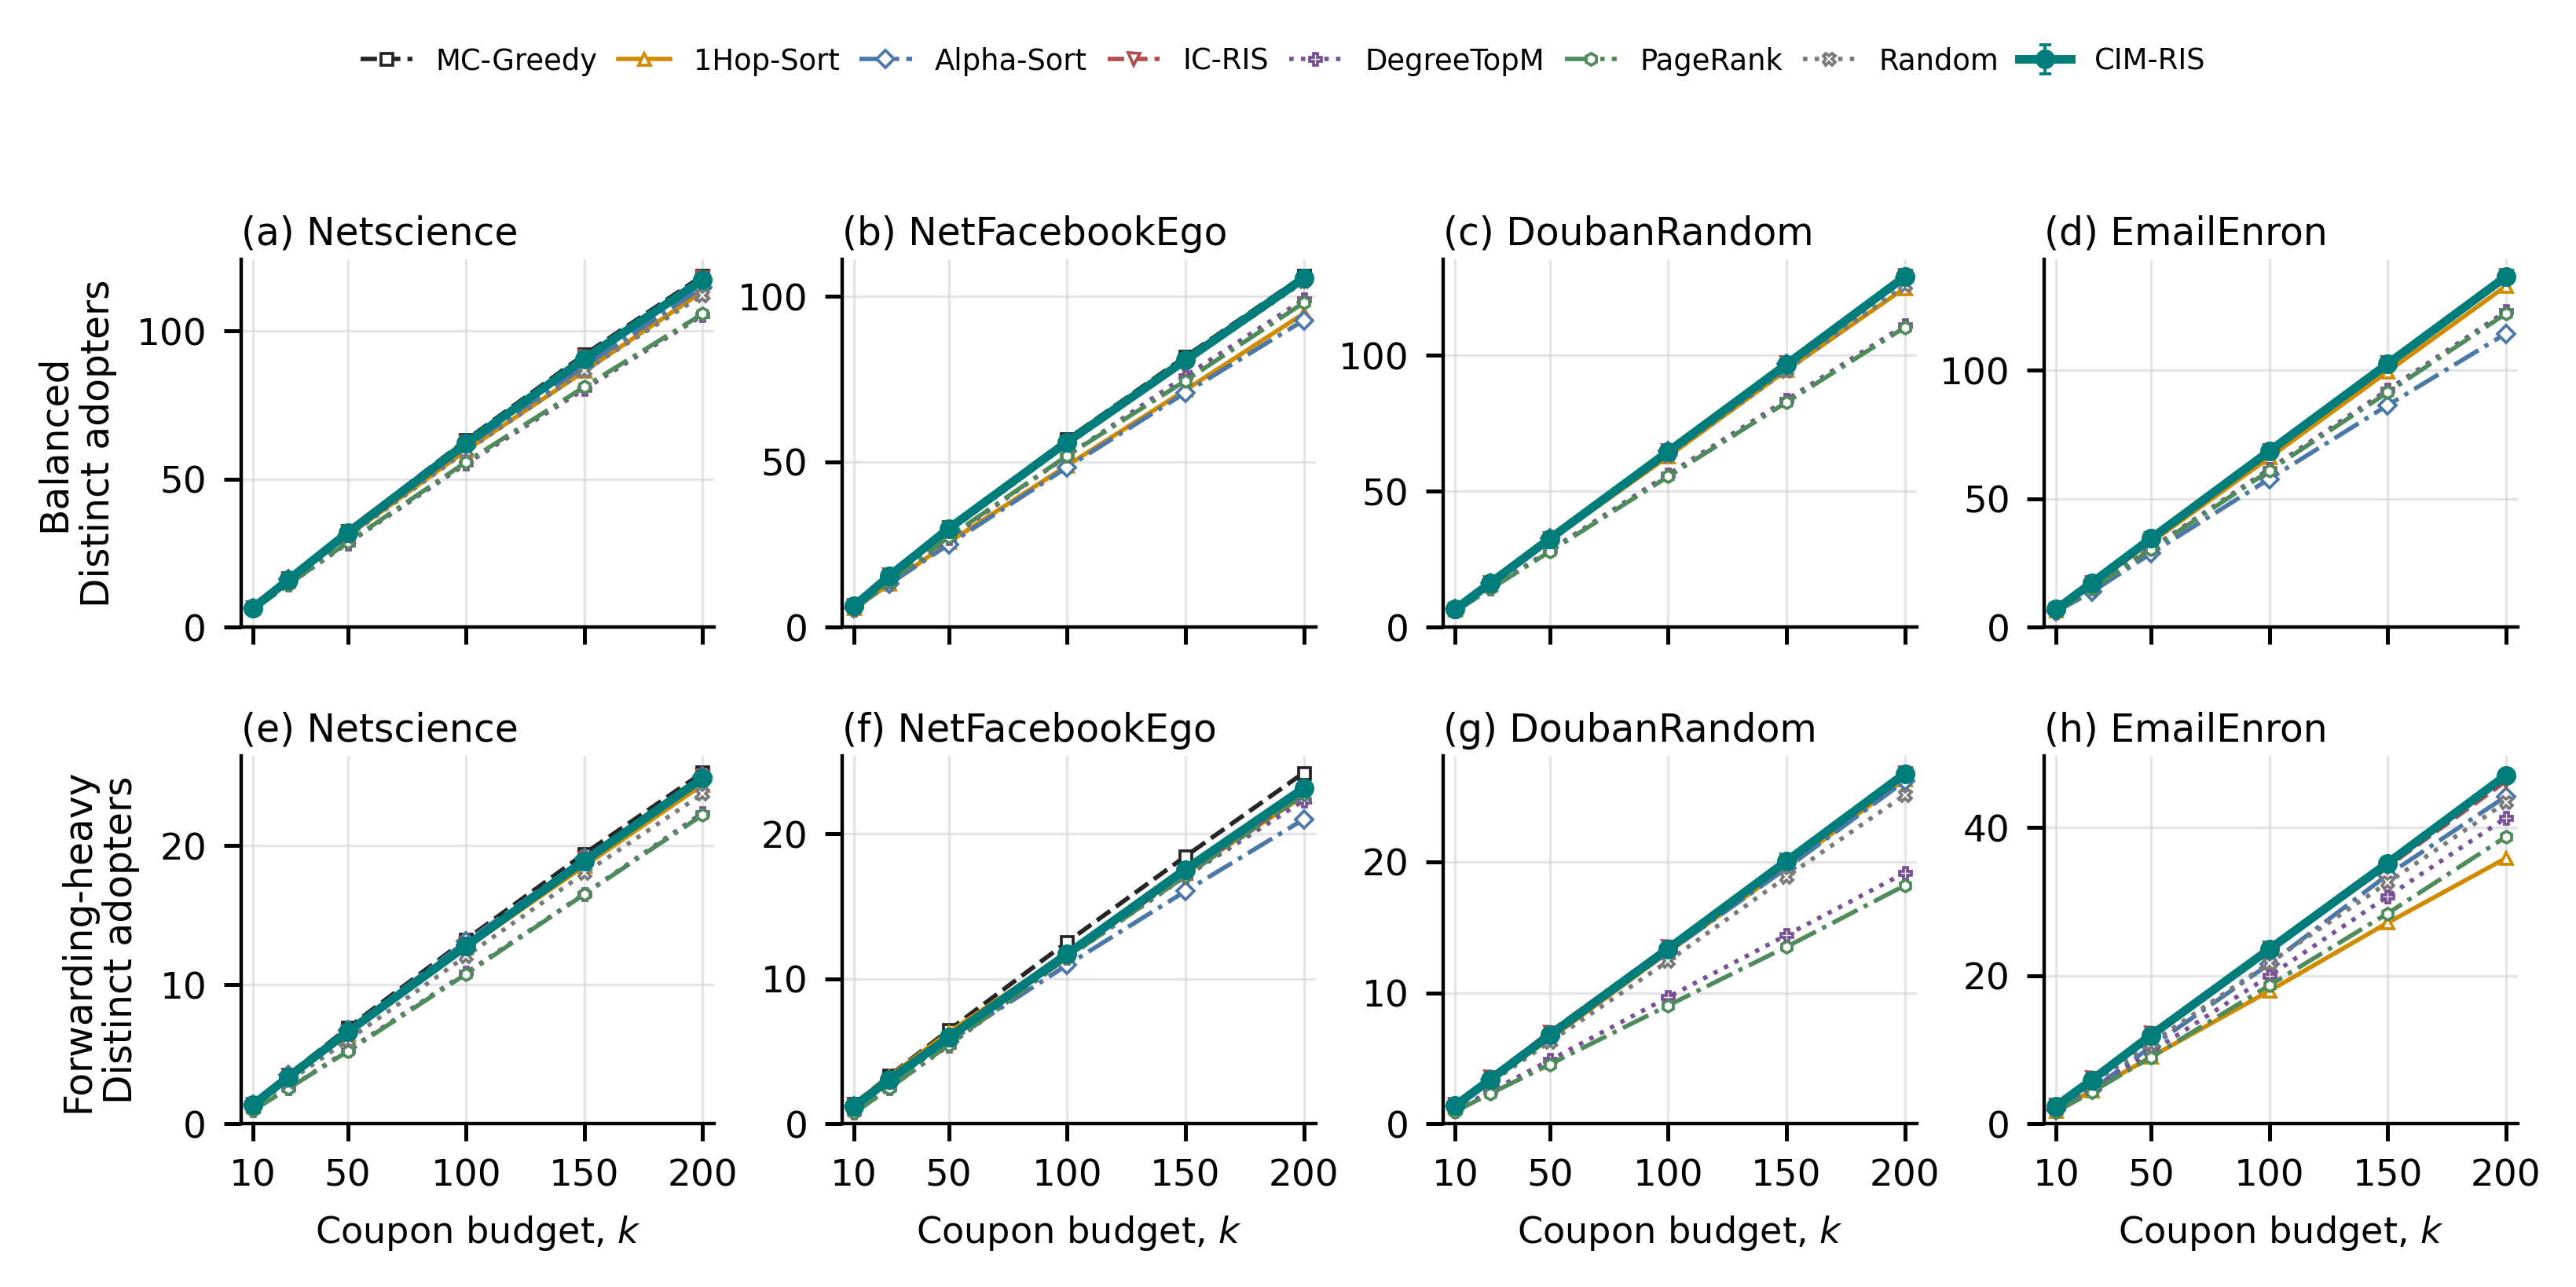
\includegraphics[width=0.87\textwidth]{figures/experiments/evidence-20260913/validated_quality_combined}
  \caption{均衡（上排）和转发主导（下排）场景的采纳规模。每个点为五次选择运行的均值，每次分配用 $10{,}000$ 个前向实现评估；\CIMRIS{} 误差条为跨运行的双侧 95\% Student-t 置信区间（自由度 4）。MC-Greedy 结果覆盖 Netscience 和 NetFacebookEgo。}
  \Description{八个折线图比较四个网络、两种扩散场景中不同采纳用户数随优惠券预算的变化。}
  \label{fig:real-quality}
\end{figure*}

\subsection{解质量}
\label{sec:exp-quality}

表~\ref{tab:aggregate-quality} 汇总了三种场景中 \CIMRIS{} 相对各基线的平均相对差异。
对于每个图--预算组合，相对差异定义为 $100(\bar{\sigma}_{\mathrm{CIM\text{-}RIS}}-\bar{\sigma}_{\mathrm{base}})/\bar{\sigma}_{\mathrm{base}}$。
该表补充图~\ref{fig:real-quality} 中各预算下的结果，并在不额外增加四面板图的情况下报告采纳主导场景。

\begin{table}[t]
  \caption{\CIMRIS{} 相对各基线的平均采纳规模差异（\%）。正值有利于 \CIMRIS{}。每种场景的基线比较对 24 个图--预算组合求平均；MC-Greedy 列对 Netscience 的六个预算求平均。}
  \label{tab:aggregate-quality}
  \centering
  \resizebox{\columnwidth}{!}{%
  \begin{tabular}{lrrrrr}
    \toprule
    场景 & MC-Greedy & 1Hop-Sort & IC-RIS & DegreeTopM & PageRank \\
    \midrule
    均衡         & $-2.3$ & $+5.8$ & $-0.1$ & $+12.6$ & $+13.3$ \\
    采纳主导   & $-2.3$ & $-0.6$ & $+1.4$ & $ +9.5$ & $ +8.9$ \\
    转发主导 & $-3.4$ & $+8.5$ & $-0.7$ & $+25.5$ & $+30.2$ \\
    \bottomrule
  \end{tabular}}
\end{table}

图~\ref{fig:real-quality} 上排展示均衡场景中各预算下的采纳规模。
在 Netscience 的全部六个预算上，\CIMRIS{} 与 MC-Greedy 参考的差距为 $1.1$--$3.8\%$，平均为 $2.3\%$。
在四个解质量图的 24 个图--预算组合中，\CIMRIS{} 在 23 个组合上优于 1Hop-Sort，平均相对提升为 $5.8\%$。
它在全部组合上优于 DegreeTopM 和 PageRank，平均提升分别为 $12.6\%$ 和 $13.3\%$。
该场景下 IC-RIS 与其基本持平：双方各在 24 个组合中的 12 个取得更高均值，平均差异为 IC-RIS 领先 $0.1\%$。
这一结果与均衡参数一致：即时采纳较常见，局部分数已能提供有效种子信息。
次要核销指标也表明，不同采纳用户目标不能与优惠券利用率互换。
例如，在 NetFacebookEgo 上 $k=200$ 时，\CIMRIS{} 平均产生 128.8 次核销，但只有 105.4 名不同采纳用户；重复核销占已核销优惠券的 $18.1\%$。

图~\ref{fig:real-quality} 下排展示转发主导压力测试。
由于访问节点时采纳较少发生，绝对采纳规模较低。
在 Netscience 上，与 MC-Greedy 的平均差距为 $3.4\%$，在 $k=200$ 时降至 $1.5\%$。
在全部图--预算组合中，\CIMRIS{} 在 24 个点中的 20 个优于 1Hop-Sort，平均提升为 $8.5\%$。
相对 DegreeTopM 和 PageRank 的平均提升分别增至 $25.5\%$ 和 $30.2\%$，且对两者均赢得全部 24 次比较。
IC-RIS 仍具竞争力，平均高出 $0.7\%$，说明在固定样本预算下，模型忠实性并不意味着经验结果始终占优。
采纳主导场景呈现另一种模式：Netscience 上与 MC-Greedy 的平均差距为 $2.3\%$；\CIMRIS{} 在 24 个点中的 23 个优于 IC-RIS，平均提升 $1.4\%$。
它再次在全部 24 个点上优于两种仅依赖拓扑的排序，但当即时采纳占主导时，1Hop-Sort 平均高出 $0.6\%$。

\begin{figure*}[t]
  \centering
  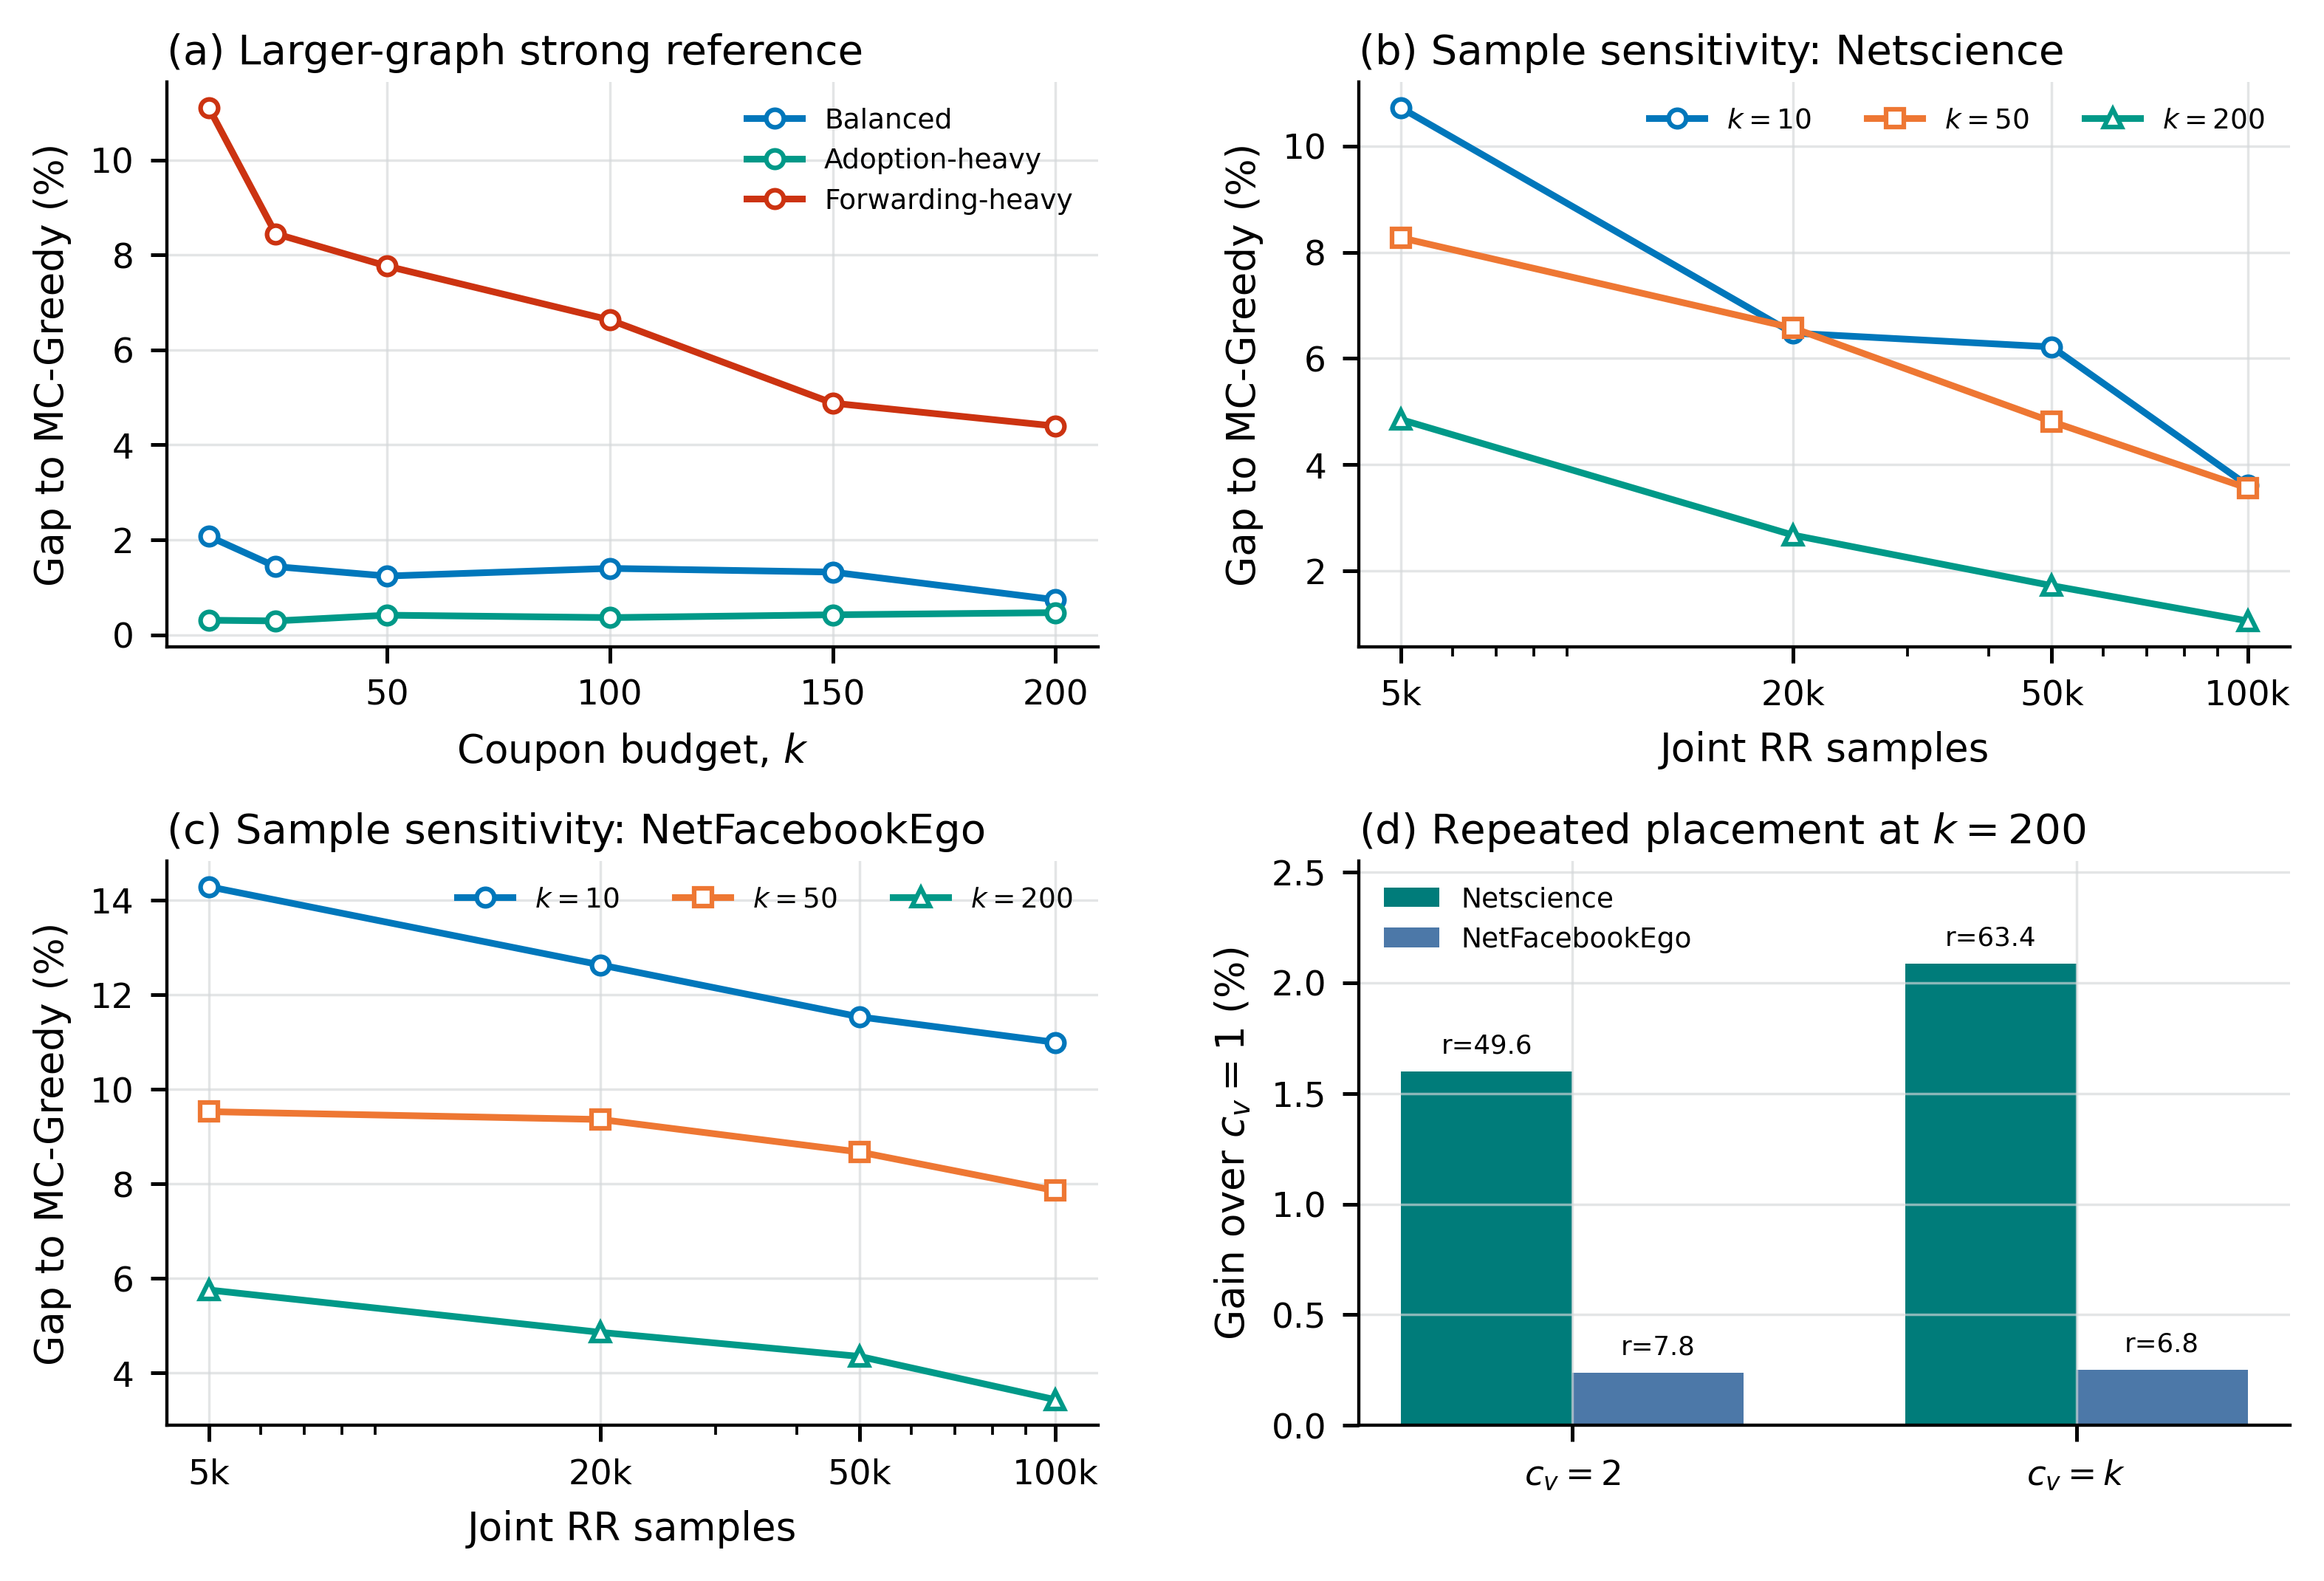
\includegraphics[width=0.91\textwidth]{figures/experiments/validated_extension_evidence}
  \caption{强参考与稳健性结果。（a）NetFacebookEgo 上与 MC-Greedy 的差距。（b--c）转发主导场景中联合 RR 样本量的影响。（d）$k=200$ 时放宽节点容量的采纳规模收益，标注为平均重复投放次数。每项统计汇总五个 \CIMRIS{} 选择随机种子，每个分配用 $10{,}000$ 个前向实现评估。}
  \Description{四个面板展示 NetFacebookEgo 上与蒙特卡洛贪心的差距、两个网络上的样本量敏感性，以及允许重复投放的收益。}
  \label{fig:extension-evidence}
\end{figure*}

\subsection{强参考比较、采样敏感性与容量}
\label{sec:exp-robustness}

我们使用每个源节点 $50{,}000$ 条独立轨迹，将强参考比较从 Netscience 扩展至 NetFacebookEgo。
图~\ref{fig:extension-evidence}(a) 显示，均衡和采纳主导场景的平均差距分别为 $1.37\%$ 和 $0.38\%$。
转发主导场景更困难：差距从 $k=10$ 时的 $11.1\%$ 降至 $k=200$ 时的 $4.4\%$，平均为 $7.2\%$。
在两个参考图、三种场景和六个预算上，观察到的差距范围为 $0.3\%$ 至 $11.1\%$。
这些结果使强参考比较不再局限于小型 Netscience 图，同时也说明，低预算、低采纳概率扩散是固定经验采样预算下最不利的情形。

图~\ref{fig:extension-evidence}(b) 和图~\ref{fig:extension-evidence}(c) 在保持评估随机流不变的条件下，改变转发主导场景的联合 RR 样本量。
对两个图与 $k\in\{10,50,200\}$ 的每种组合，将样本量从 $5{,}000$ 增至 $100{,}000$ 均降低了与 MC-Greedy 的平均差距。
六种组合的平均差距从 $8.90\%$ 降至 $5.09\%$。
改善最大的是 Netscience 的 $k=10$，差距从 $10.72\%$ 降至 $3.61\%$；NetFacebookEgo 的 $k=10$ 仍最困难，差距从 $14.29\%$ 降至 $11.00\%$。
因此，采样预算解释了部分、但并非全部与 MC-Greedy 的剩余差距。
相应运行时间体现了成本与精度的权衡。
对六个网络--预算组合求平均，样本量为 $5{,}000$、$20{,}000$、$50{,}000$ 和 $100{,}000$ 时，选择时间分别为 $0.266$、$1.016$、$2.435$ 和 $4.741$ 秒。
对应平均差距分别为 $8.90\%$、$7.10\%$、$6.22\%$ 和 $5.09\%$。
运行时间大致正比于样本量，而观察到的质量改善呈现边际收益递减。
这一权衡为主比较中的固定两级方案提供了动机，但不会使经验方案自动成为理论标定的样本量 $T$。

最后，图~\ref{fig:extension-evidence}(d) 在 $k=200$ 时比较 $c_v=1$、$c_v=2$ 和 $c_v=k$ 的容量设置。
在均衡和采纳主导场景，即使允许重复投放，\CIMRIS{} 和 MC-Greedy 也几乎总是选择不同种子，因此放宽容量没有实质影响。
在转发主导场景，\CIMRIS{} 在 Netscience 平均采用 $49.6$--$63.4$ 次重复投放，采纳规模相对 $c_v=1$ 提高 $1.60$--$2.09\%$；在 NetFacebookEgo 平均采用 $6.8$--$7.8$ 次重复投放，采纳规模提高约 $0.25\%$。
因此，当较长轨迹使少数源节点反复具有投放价值时，重复投放可能有用，但其收益并不适用于所有扩散场景。

\FloatBarrier

\subsection{条件采样与可扩展性}
\label{sec:exp-efficiency}

图~\ref{fig:real-sampler} 单独考察转发主导场景下的条件根采样器。
在 $k=10$ 时，均匀根采样在 Netscience 的 $68.4\%$ 样本及 EmailEnron 的 $61.0\%$ 样本中没有任何根采纳门控触发。
条件采样消除了这些工作，使 Netscience 的变异系数从 $0.128$ 降至 $0.087$，EmailEnron 从 $0.809$ 降至 $0.492$。
本轮补充实验完整保存两图、三个预算、两种采样器的共 360 个批次，包括每批随机种子、估计值、零贡献比例及耗时。
采用相同选择结果和采样随机种子时，估计均值与标准差复现了历史汇总。
完整批次计时包含根权重与根节点列表生成、门控采样及反向遍历，不含图加载；本轮测量在 Windows、Python~3.12.8、NumPy~2.2.4 环境下单进程执行，不与原 Linux 选择时间直接比较。
在这一计时范围下，$k=10$ 时相应方差--时间效率提升为 $1.20\times$ 和 $1.37\times$。
在全部六个测量条件中，该比值介于 $1.20\times$ 与 $1.61\times$，均有利于条件采样。
但在 $k=200$ 时，均匀根样本中没有门控触发的比例已低于 $0.3\%$，因此解释经验方差差异时须考虑仅有 30 个批次的有限样本规模。

\begin{figure}[t]
  \centering
  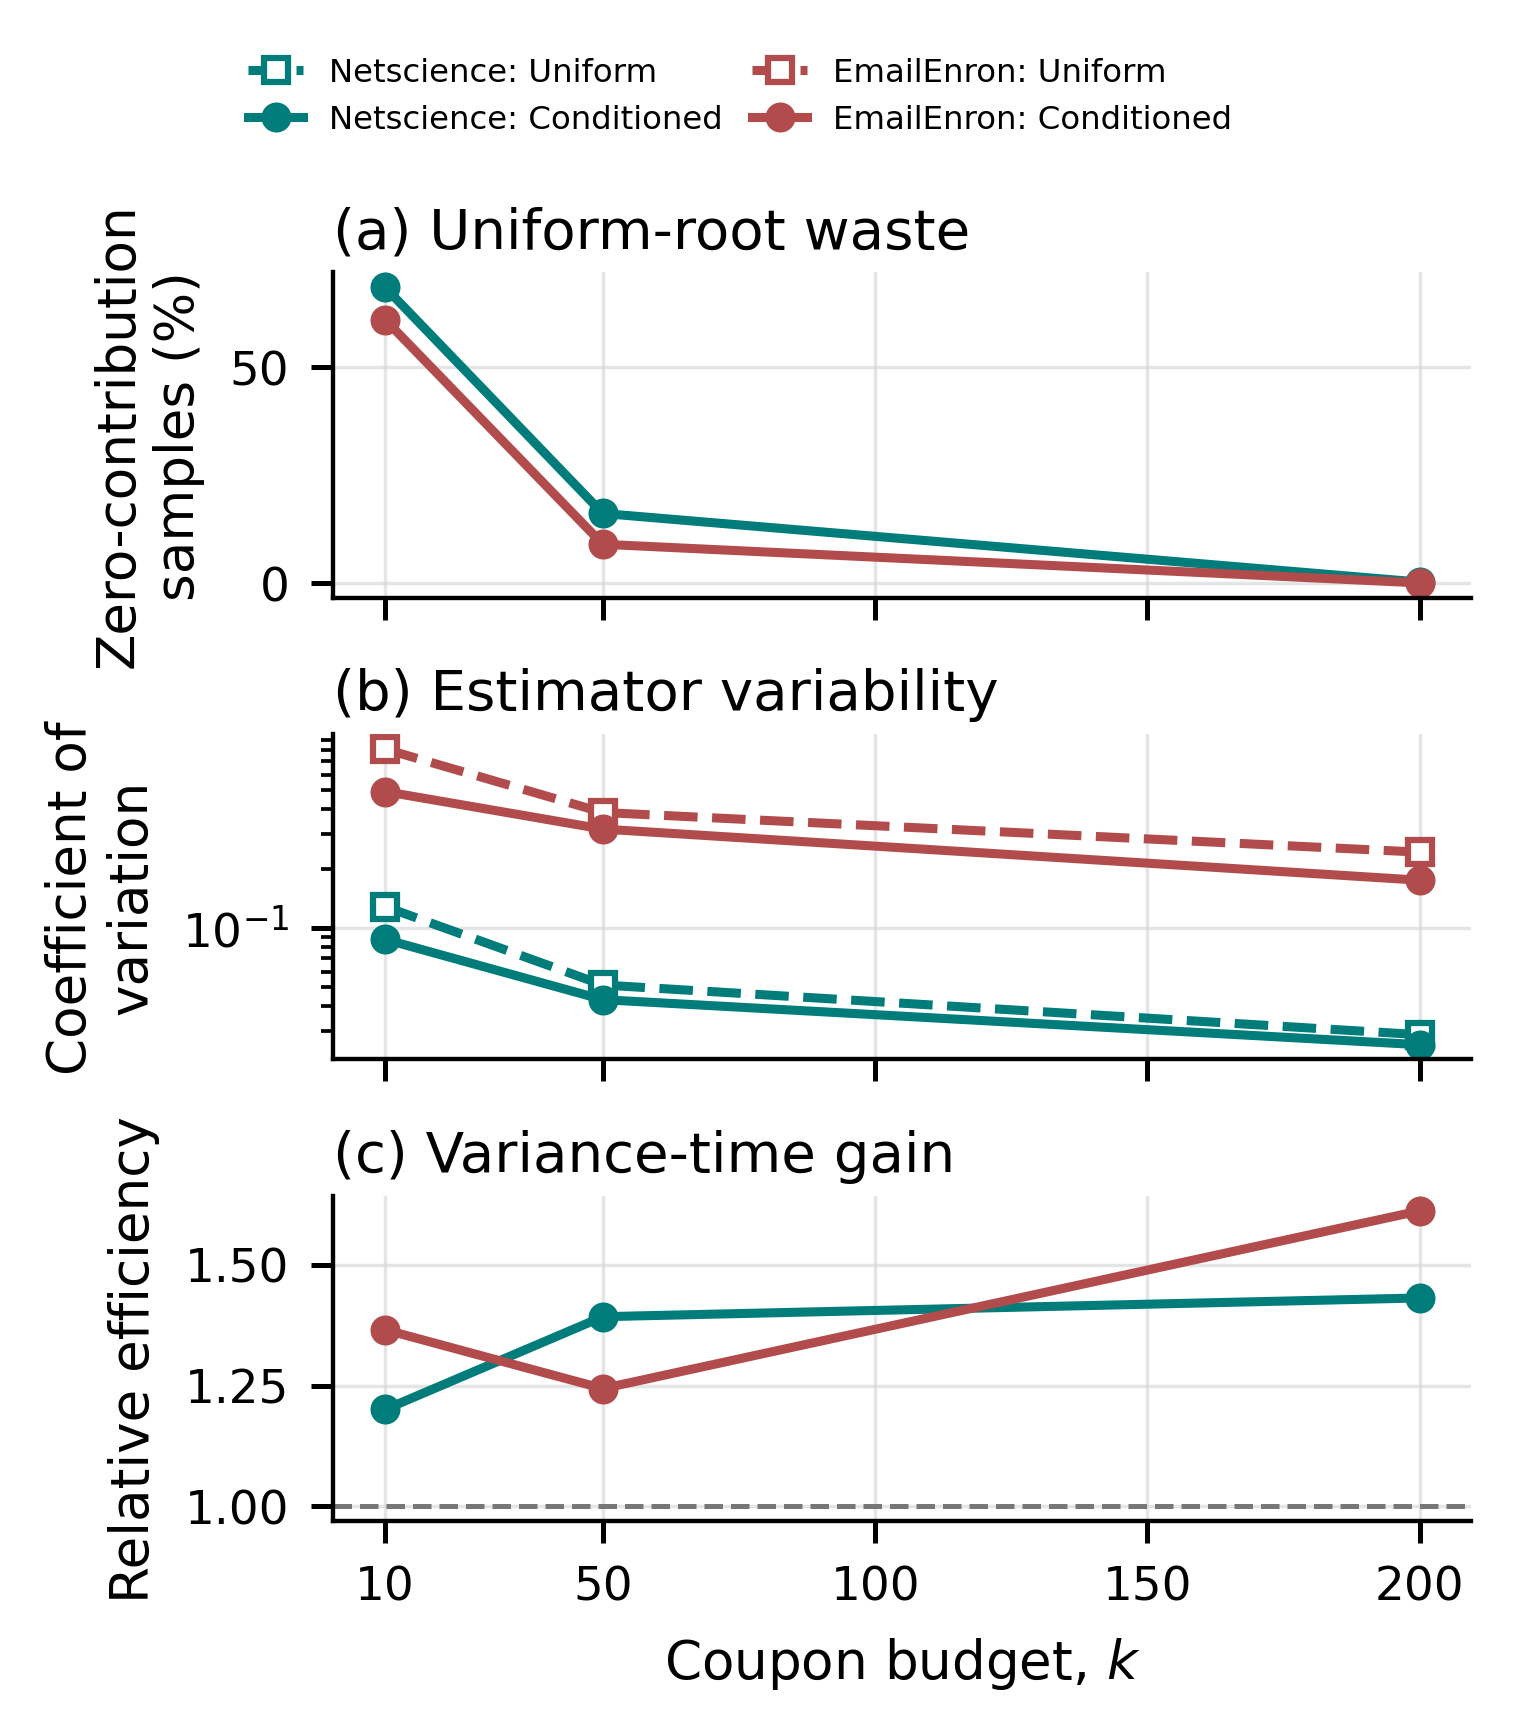
\includegraphics[width=\columnwidth]{figures/experiments/evidence-20260913/validated_sampler_ablation}
  \caption{转发主导场景中的均匀根与条件根估计。每项统计采用 30 个独立批次，每批 $20{,}000$ 个样本。相对效率为均匀与条件采样的方差--时间乘积之比，大于一表示条件采样更优；时间计入根节点生成，每批原始结果均保留。}
  \Description{三个面板比较 Netscience 和 EmailEnron 上两种根采样的零贡献样本、变异系数及方差--时间效率。}
  \label{fig:real-sampler}
\end{figure}

\begin{figure}[t]
  \centering
  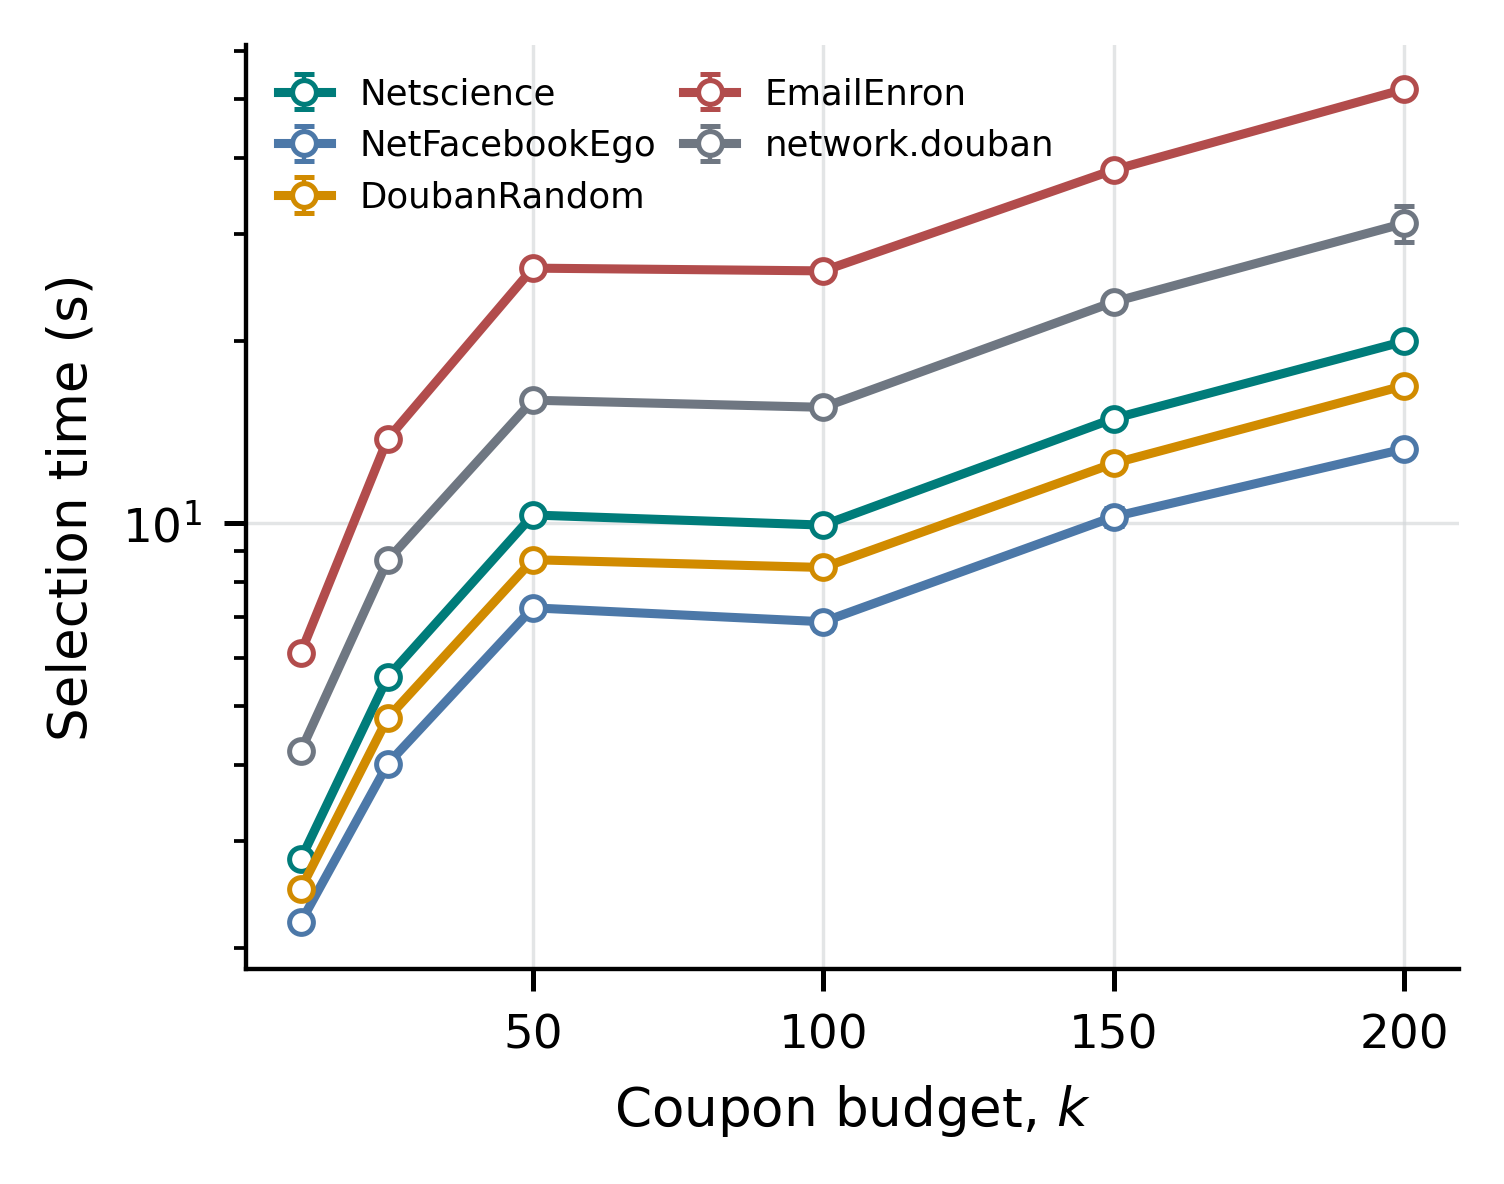
\includegraphics[width=\columnwidth]{figures/experiments/validated_runtime_scalability}
  \caption{均衡场景中单进程 \CIMRIS{} 选择时间，为五次运行均值。$k\leq50$ 时样本预算为 $100{,}000$，$k\geq100$ 时为 $50{,}000$；误差条为一个标准差。}
  \Description{折线图以对数纵轴展示五个图实例的选择时间随优惠券预算的变化。}
  \label{fig:real-runtime}
\end{figure}

图~\ref{fig:real-runtime} 报告 \CIMRIS{} 的端到端选择时间，包括样本生成和贪心覆盖。
若干图从 $k=50$ 到 $k=100$ 时耗时下降，是预先设定的采样预算减半所致，并非单样本计算变快。
在 $k=200$ 时，EmailEnron 的平均选择时间为 51.9 秒，规模更大的 network.douban 为 31.2 秒。
不同真实图的时间排序并不随规模单调变化，反映了度分布和 RR 集大小的差异。
因此，该结果应理解为实际可扩展性证据，而非最坏情况复杂度界的直接经验拟合。

\subsection{完整 Douban 的独立质量评估}
\label{sec:exp-large-quality}

为补足大图实验原先只有选择耗时、缺少独立质量评估的证据，我们在完整 network.douban 上开展补充实验。
沿用均衡场景、六个预算 $k\in\{10,25,50,100,150,200\}$、五个选择随机种子以及主实验的两级 RR 预算，比较 \CIMRIS{}、IC-RIS、1Hop-Sort、Alpha-Sort、DegreeTopM、PageRank 和 Random。
每个分配用与选择独立的 $10{,}000$ 个新前向实现评估，同一配置内各方法共用评估随机流。
共保存 30 个任务、210 个方法分配及其统计；每个任务均记录实际种子分配、随机流标识、代码和图文件哈希。
\CIMRIS{} 的样本内估计及 RR 成员数复现了原可扩展性记录，但样本内估计仅作诊断，不作为所选分配的质量估计。
补充实验与本轮采样消融使用相同的 Windows/Python 环境，新记录的耗时不替换图~\ref{fig:real-runtime} 中的历史 Linux 耗时。

\begin{figure*}[t]
  \centering
  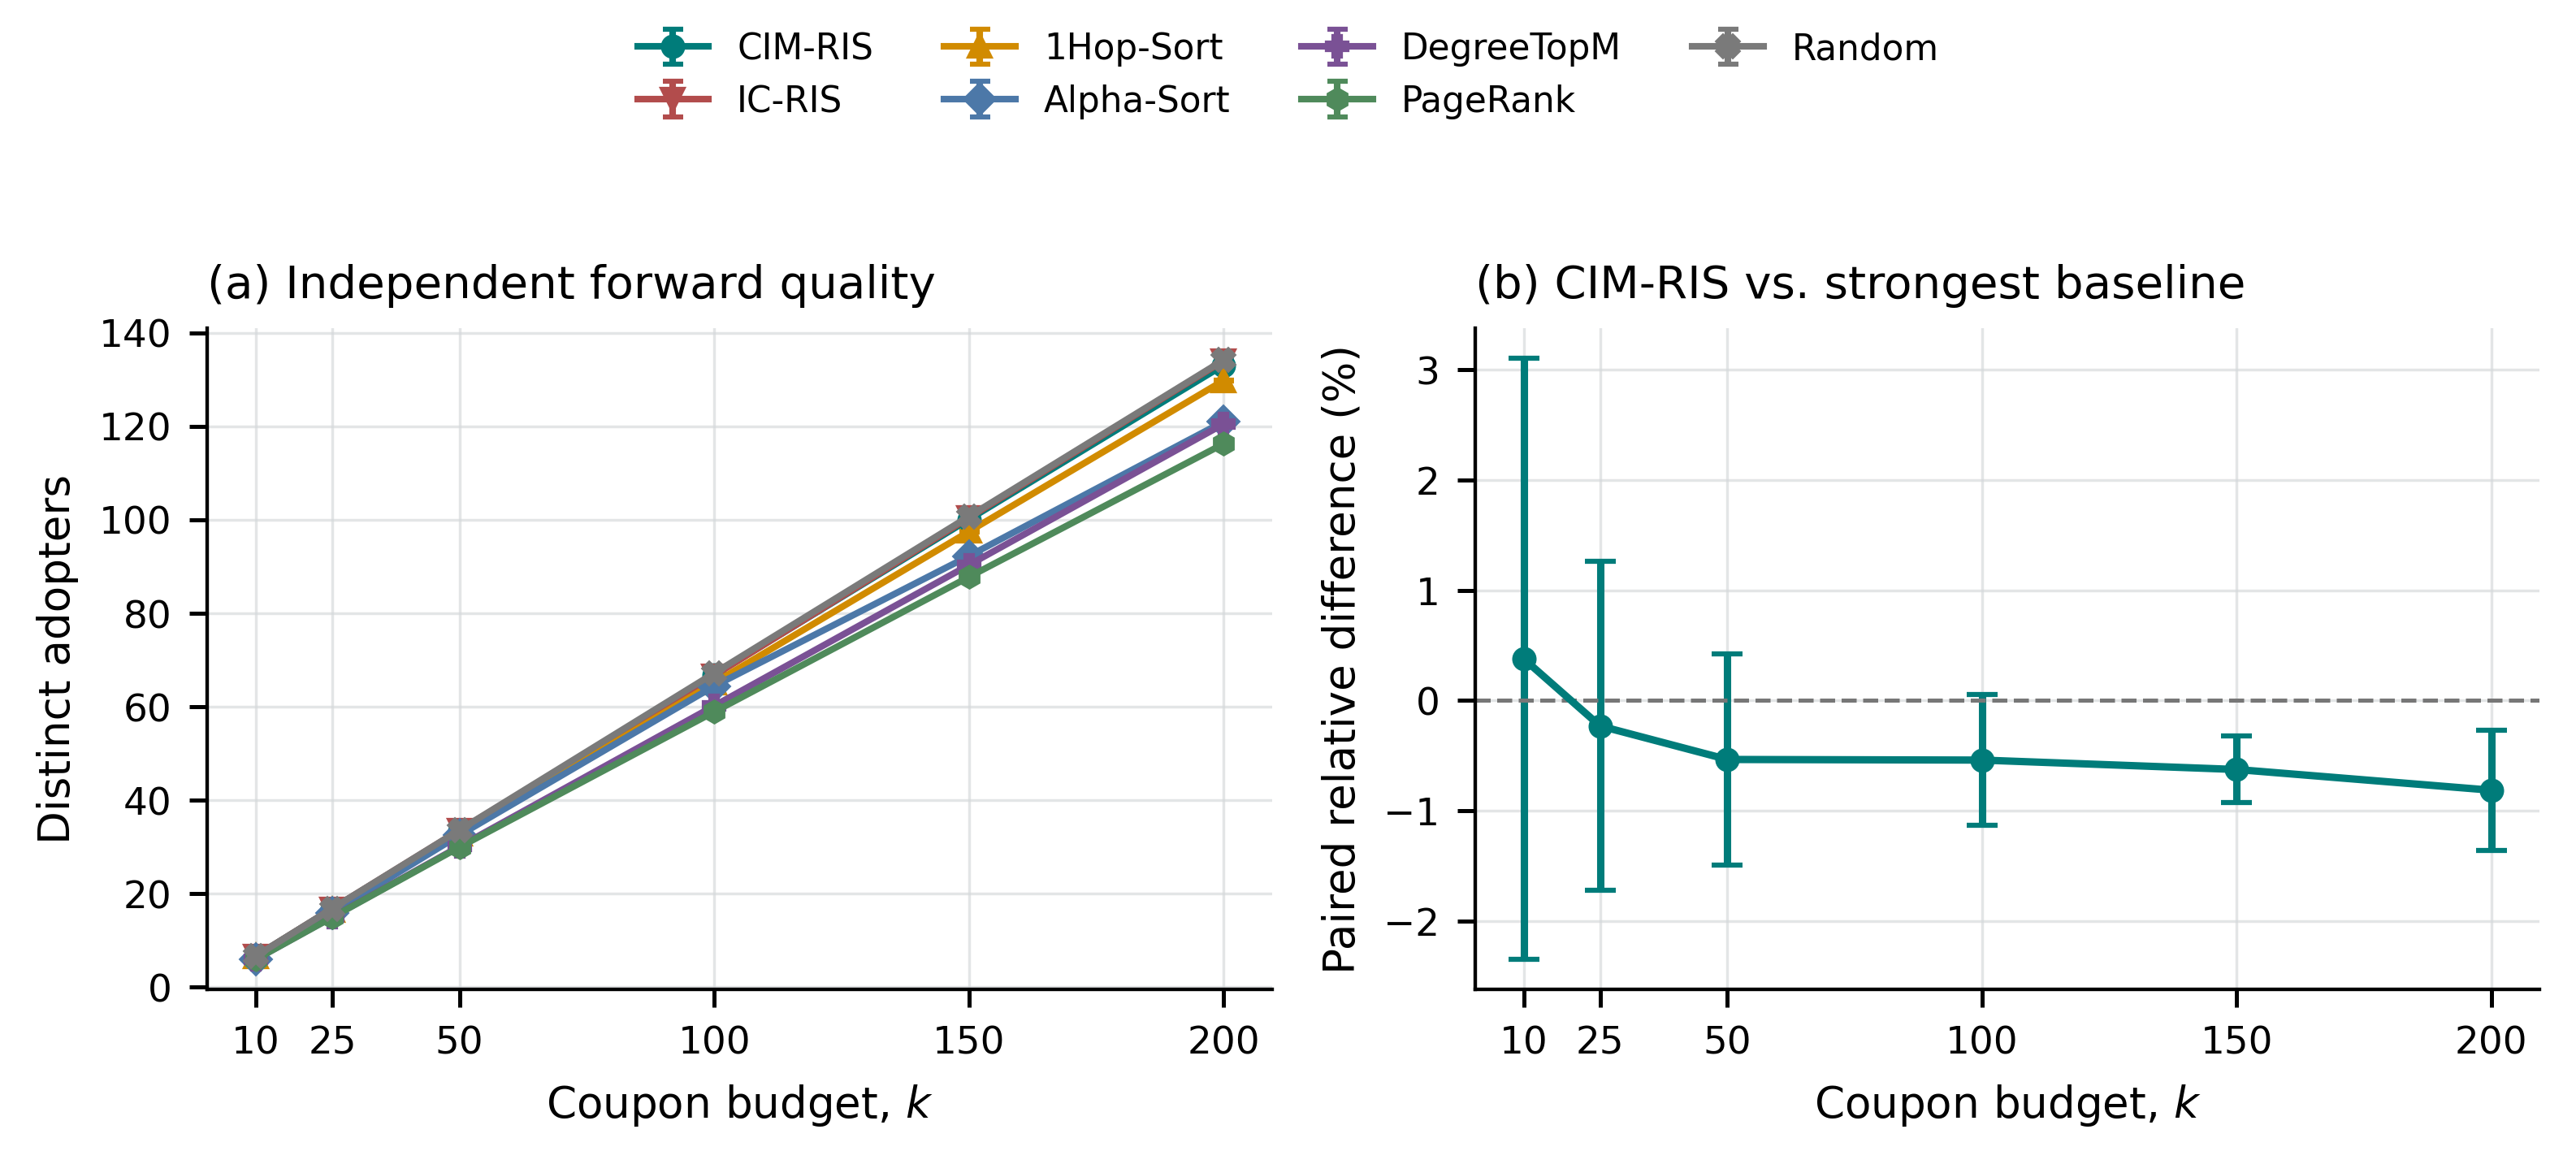
\includegraphics[width=0.95\textwidth]{figures/experiments/evidence-20260913/large_graph_quality}
  \caption{完整 Douban 在均衡场景下的独立质量评估。（a）不同核销用户数，误差条为五次运行的双侧 95\% Student-t 区间。（b）\CIMRIS{} 相对各预算下平均采纳规模最高基线的配对相对差异，误差条由五个配对差异计算。基线根据同一组观测选择，因此区间用于描述变异，不表示经过选择或多重比较校正的显著性结论。}
  \Description{左图展示七种方法随优惠券预算的独立采纳规模；右图保留相对最强基线的正负差异，较大预算下随机投放具有更高均值。}
  \label{fig:large-independent-quality}
\end{figure*}

图~\ref{fig:large-independent-quality} 显示，大图上的快速选择并不自动带来最优的经验质量。
在 $k=10$ 时，\CIMRIS{} 的平均采纳规模为 $6.7063$，最强基线 IC-RIS 为 $6.6826$，均值相对差异约为 $+0.36\%$。
在 $k=25,50,100,150,200$ 时，平均表现最高的基线均为 Random，\CIMRIS{} 相对其均值的差异分别为 $-0.24\%$、$-0.54\%$、$-0.54\%$、$-0.63\%$ 和 $-0.81\%$。
特别地，$k=200$ 时二者的平均不同核销用户数为 $133.0522$ 和 $134.1437$。
这些结果支持固定经验采样预算下质量优势具有条件性的结论，不能将主实验中对拓扑排序的优势外推为对大图上所有简单策略的优势。
本补充实验仅覆盖均衡场景，没有构建完整大图的 MC-Greedy 或精确最优参考，也未验证理论样本量要求，因此不能据此声称测得了对最优解的近似比。

%% ============================================================
%% 7. CONCLUSION
%% ============================================================
\section{结论}
\label{sec:conclusion}

本文形式化研究了不可复制、单路径扩散下的优惠券影响力最大化。
在该模型中，优惠券被核销、丢弃或转发给一个邻居，且只有核销产生采纳用户。
通过节点容量，分配形式同时支持不同种子和重复投放，并对每个采纳用户仅计数一次。
我们证明 CIM 是 NP-hard 的，且采纳规模在优惠券分配上具有单调性和 DR 次模性。
随后构造 $k$ 联合 RR 样本，利用其覆盖事件无偏估计采纳规模和边际收益。
由此得到的 \CIMRIS{} 算法以高概率实现 $(1-1/e-\epsilon)$ 近似；当预算、精度和采纳规模下界固定时，其期望运行时间关于图规模近线性。
在两个参考图、三种场景中，实验结果与高精度蒙特卡洛贪心的差距为 $0.3$--$11.1\%$；最大差距出现在 NetFacebookEgo 的低预算、转发主导配置，并随 RR 样本预算增加而下降。
在三种场景的全部 72 个图--预算组合中，\CIMRIS{} 均优于 DegreeTopM 和 PageRank，最大平均提升出现在转发主导场景。
局部基线和广播基线在部分实例上仍具竞争力，没有方法在所有图和预算上占优。
完整 Douban 的补充独立评估进一步发现，在所测试的六个预算中，Random 在五个预算上的均值略高于 \CIMRIS{}，差异为 $0.24\%$--$0.81\%$；实际可扩展性与相对解质量应分别评估。
条件根采样消除零贡献样本；计入根节点生成的补充测量中，两个测试图在 $k=10$ 时分别获得 $1.20\times$ 和 $1.37\times$ 的方差--时间效率提升。
容量实验进一步表明，重复投放在转发主导场景带来小幅收益，但在采纳较常见时很少被选择。

仍有若干方向值得研究。
第一，可将模型扩展至\emph{自适应}分配，使后续投放依赖已观测的早期采纳，从而减少时效性活动中的预算浪费。
第二，每个账户仅核销一次、采纳后仍存在转发激励等耦合活动规则，需要在 RR 样本中编码到达顺序和用户状态。
第三，更紧的下界估计及针对极低采纳概率的方差降低方法，有望进一步降低 \CIMRIS{} 的实际成本。

\appendix
\section{补充参数区域实验}
\label{app:parameter-sweep}

主评估的三种场景提供了具有代表性的运行点，但未展示场景之间的相对表现如何变化。
因此，我们在 Netscience 和 NetFacebookEgo 上开展预先规定的二维参数扫描。
该实验旨在刻画有利及不利区域，而非证明 \CIMRIS{} 优于所有替代方法。

令 $\hat d_u\in[0,1]$ 为节点 $u$ 的归一化对数度。
给定中心核销份额 $r$ 和转发概率 $t$，设置
\[
\begin{aligned}
  h_u &=
    \operatorname{clip}\!\left(r+0.20(0.5-\hat d_u),0.05,0.95\right),\\
  p_u^a&=(1-t)h_u,\qquad
  p_u^d=(1-t)(1-h_u),\qquad
  p_u^t=t.
\end{aligned}
\]
因此，$h_u$ 控制停止传播条件下的核销概率，$t$ 控制优惠券游走的持续程度。
孤立节点的转发概率质量转移给丢弃。
完整网格在 $k=100$ 时采用 $t\in\{0.30,0.50,0.70,0.85,0.93\}$ 和 $r\in\{0.20,0.40,0.60,0.80\}$。
此外固定 $r=0.60$，在全部五个转发概率下评估 $k\in\{25,100,200\}$。
每种配置采用五个选择随机种子及相同的不同种子策略。
固定低 RR 预算可能使自适应贪心选择过拟合，因此每次 \CIMRIS{} 运行从 $100{,}000$ 个嵌套条件样本开始，逐步将样本前缀加倍。
最小终止预算取以下两者的较小值：$1.5$ 百万个样本，以及为每个优惠券索引和候选节点提供十次期望非空 RR 观测所需、并向上取整至 $50{,}000$ 整数倍的预算。
达到该下限后，用 $5{,}000$ 个新的配对前向实现比较连续两次分配，当采纳规模的相对差异不超过 $0.5\%$ 时停止，或在达到 $3$ 百万样本硬上限时停止。
IC-RIS 获得与 \CIMRIS{} 相同的最终 RR 样本量。
最终结果使用 $10{,}000$ 个新的前向实现，与选择及稳定性验证均独立。
比较包含 IC-RIS、1Hop-Sort、Alpha-Sort、DegreeTopM 和 PageRank。
在每个参数单元中，\CIMRIS{} 与该单元内平均采纳规模最高的基线比较，这比使用固定基线更严格。

\begin{figure*}[t]
  \centering
  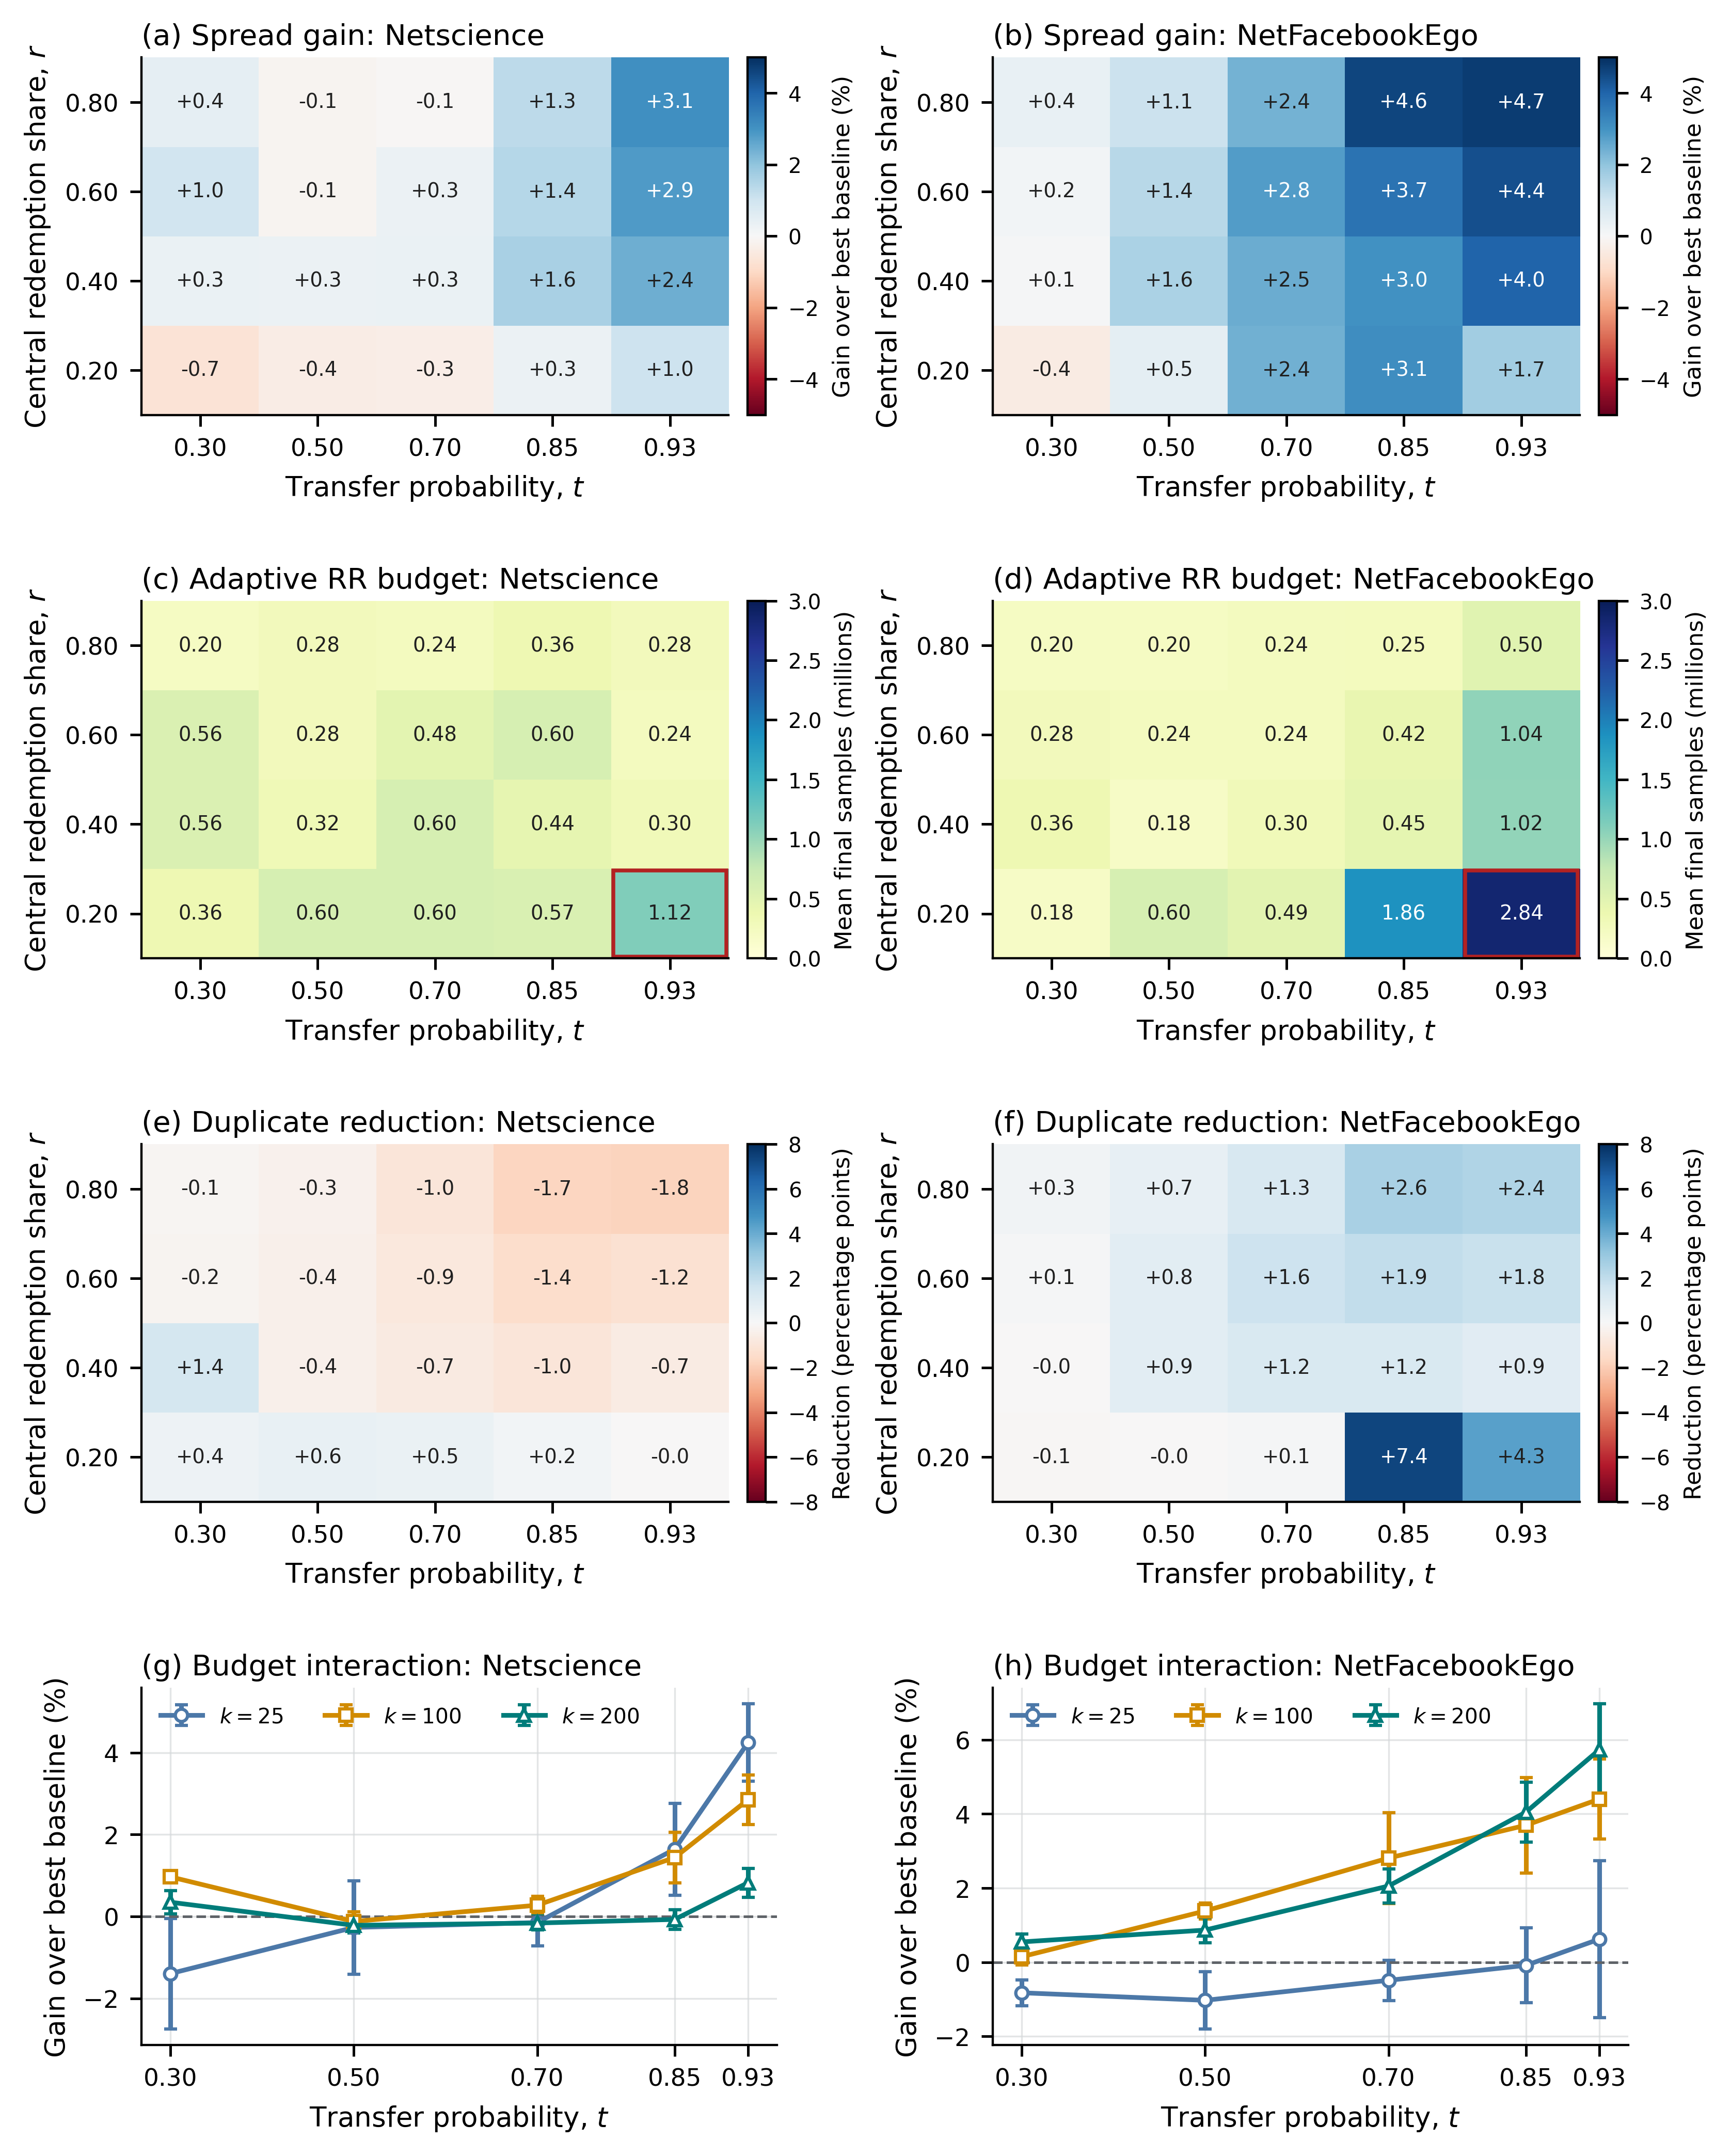
\includegraphics[width=0.96\textwidth]{figures/experiments/appendix_parameter_sweep}
  \caption{两个图实例上的完整参数区域研究。（a--b）$k=100$ 时 \CIMRIS{} 相对每个单元中最强非 oracle 基线的采纳规模差异。（c--d）自适应停止后的平均最终 RR 样本量；红框标记至少有一次运行在硬上限处仍未稳定的单元。（e--f）相对同一基线的重复核销比例降低量，正值有利于 \CIMRIS{}。（g--h）$r=0.60$ 时相对采纳规模差异随预算的变化。热力图保留全部预设单元，折线误差条为五次配对选择与评估运行的 95\% 置信区间。}
  \Description{八个面板完整展示转发概率与核销份额扫描，依次报告相对最强基线的采纳规模收益、自适应 RR 样本量、重复核销比例变化和预算交互，保留正负收益区域。}
  \label{fig:appendix-parameter-sweep}
\end{figure*}

图~\ref{fig:appendix-parameter-sweep}(a--b) 报告完整的 $k=100$ 网格。
在 NetFacebookEgo 上，\CIMRIS{} 在 20 个单元中的 19 个具有高于最强基线的平均采纳规模，平均相对差异为 $2.20\%$，最大值为 $(t,r)=(0.93,0.80)$ 处的 $4.75\%$。
唯一负收益单元为 $(0.30,0.20)$，其中 IC-RIS 高出 $0.42\%$。
在 Netscience 上，\CIMRIS{} 在 20 个单元中的 14 个均值更高，平均差异为 $0.75\%$，范围为 $-0.69\%$ 至 $3.08\%$。
在两个图的全部 40 个单元中，它均优于 DegreeTopM 和 PageRank。
因此，持续转发时优惠券感知覆盖最有利，而在若干低转发、低核销单元，简单的采纳感知排序仍具竞争力。

图~\ref{fig:appendix-parameter-sweep}(c--d) 表明，上述比较所需采样量明显高于此前固定的低预算。
全部 300 次选择运行的最终 RR 样本量中位数为 $300{,}000$，均值为 $534{,}500$。
295 次满足停止规则；11 次达到 $3$ 百万上限，其中五次仍未稳定。
这五次未解决的不稳定运行均保留在汇总结果中。
在 $k=100$ 时，最高平均终止预算为 NetFacebookEgo 的 $(0.93,0.20)$ 单元中的 $2.84$ 百万，与高转发、低核销条件下根采纳观测稀缺相一致。
这些是经验稳定性检查，并非理论层面的 $(\epsilon,\delta)$ 保证。

图~\ref{fig:appendix-parameter-sweep}(g--h) 的预算切片进一步表明，有利区域可能随活动规模变化。
在 NetFacebookEgo 上，$k=25$ 时 \CIMRIS{} 在五个转发设置中的一个均值更高，而 $k=100$ 和 $k=200$ 时均在全部五个设置中更高；相应平均差异分别为 $-0.36\%$、$2.49\%$ 和 $2.65\%$。
Netscience 的变化不具有相同单调性：对应胜出次数为二、四、二，平均差异为 $0.82\%$、$1.08\%$ 和 $0.14\%$。

最后，图~\ref{fig:appendix-parameter-sweep}(e--f) 将重复核销比例 $(\bar\rho-\bar\sigma)/\bar\rho$ 与最强基线比较。
正值表示 \CIMRIS{} 将更高比例的核销转化为不同采纳用户。
在 $k=100$ 的 40 个单元中，该改善与相对采纳规模差异的 Pearson 相关系数为 $0.43$。
因此，避免重复与测得收益相关，但不能完全解释收益；所选游走是否抵达愿意核销的用户同样重要。
\FloatBarrier
\balance

\bibliographystyle{ACM-Reference-Format}
\bibliography{references}

\end{document}
